% "Станет проще"

\documentclass[a4paper,12pt]{article} % тип документа

% report, book

%  Русский язык
\usepackage{ucs}
%\usepackage[T2A]{fontenc}			% кодировка
%\usepackage[utf8]{inputenc}			% кодировка исходного текста
\usepackage[utf8x]{inputenc}
\usepackage[english,russian]{babel}
%\usepackage{cmap}



\usepackage{graphicx}
\usepackage[english,russian]{babel}	% локализация и переносы



\usepackage[left=30mm, top=20mm, right=20mm, bottom=30mm, nohead, nofoot]{geometry}
% Математика
\usepackage{amsmath,amsfonts,amssymb,amsthm,mathtools} 
\usepackage{csvsimple}
\usepackage{multirow}


\usepackage{wasysym}
\usepackage{subcaption}
\usepackage{gensymb}
\usepackage{verbatim}
\usepackage[hidelinks]{hyperref}
\usepackage{float}
\usepackage{enumerate}
\usepackage{wrapfig}
\usepackage{listings} %написание кода
%\usepackage{times} %шрифт

\usepackage[dvipsnames]{xcolor}
\usepackage{verbatim} %comments

%Заговолок



\graphicspath{ {img/} }


\begin{titlepage}
\author{Соловьянов Михаил}
\title{Диплом \\ \LARGE{« 
»\\ 553 гр.}}
\date{\today}
\end{titlepage}



\begin{document} % начало документа

\tableofcontents
\addcontentsline{toc}{section}{.}
\newpage



\section{Вступление и актуальность темы исследования}

Растущее развитие цифровых технологий раздвигает границы потребности в хранении информации, причем важен становиться не только объем, но скорость доступа, плотность размещения элементов, а так же цена одного бита информации. В современных коммерческих энергонезивисимых  SSD (Solid State Drive) носителях скорость чтения и записи достигает 3 Гб/с \cite{ssd}.   В различных ЭВМ и цифровых приборах могут использоваться множество различных типов памяти. Среди энергонезависимых типов памяти доминирут два типа памяти: память на магнитных носителях, с высокой плотностью элементов, и низкой стоимостью одного бита информации, однако же низкой скоростью чтения и записи в виду зависимости их от механических деталей. Второй вид памяти доминирующий на рынке энергонезависимой памяти: eFlash память, и ее родственники. В таблице  \eqref{tab:memory} приведено сравнение различных типов памяти, как энергозависимых, так и энергонезависимых. Как можно заметить, главным недостатком eFlash помимо относительной цены за бит является существенно ограниченное количество битов которые могут быть перезаписаны в ячейку. В целом это число не превышает $10^5 $ Для наиболее доступной памяти это обычно $ 10^3-10^4  $ циклов записи. При этом существует потребность в носителях которые могли бы постоянно и быстро записывать большие объемы данных. 
%Таблица с типами памяти.

\begin{table}[h]
\centering
\begin{tabular}{|l|l|l|l|}
\hline
                          & FRAM            & DRAM       & eFLASH     \\ \hline
Циклов чтения             & $>10^{15}$      & $>10^{15}$ & $>10^{15}$ \\ \hline
Циклов записи             &  \textcolor{ForestGreen}{$>10^{15}$}      & $>10^{15}$ &\textcolor{BrickRed} {$\approx 10^6$}    \\ \hline
Напряжение записи         & \textcolor{ForestGreen}{$V_c \approx V_{dd} $} & $V_{dd} $  &\textcolor{BrickRed}{ 10-18В }    \\ \hline
Время хранения информации & >5ти лет        & --         &>5ти лет   \\ \hline
Время записи              & 20-60нс         & 20-60 нс   & 1 мкС      \\ \hline
Время чтения              & 45-60нс         & 45-60 нс   & 50-70 нс   \\ \hline
\end{tabular}
\caption{Сравнение FRAM,DRAM,eFLASH памяти \cite{FRAM}.}
\label{tab:memory}
\end{table}

Исследования проводимые в лаборатории нейровычислительных систем мфти в рамках разработки интегральных схем для анализа работы мозга требуют реализации энергонезависимой и энергоэффективной памяти интегрированной в чип, при этом способной записывать многократно большие объемы данных. Приняв во внимание исследования сделанные в ЦКП МФТИ в течении последних 5ти лет \cite{Segneto_MIPT-I}\cite{Segneto_MIPT-II}\cite{Segneto_MIPT-III} позволяют сделать вывод о возможности реализации нового поколения динамической памяти на основе конденсаторов из сегнетоэлектрика. Патенты на реализацию такой памяти были получены еще в СССР в 70-х годах \cite{patent}. Первые образцы же  такой памяти производились еще в ссср в 80х, однако бурный рост eFlash технологий, вместе со сложностью использований прошлого поколения сегнетоэлектрика в производстве привела сперва к ограниченному коммерческому использованию а затем и к упадку данной технологии. Однако недавние открытия в области сегнетоэлектрических свойств уже интегрированного в техпроцесс хай К деилектрика (Оксида Гафния) вполне возможно являются прелюдией к революции в области энергонезависимой памяти. В стенах лаборатории нейровычислительных систем планируется разработать и испытать данную память для реализации хранения информации на чипе используемым внутри организма для считывания сигналов мозга. К такой памяти предьявляются требования по низкому энергопотреблению и высокой скорости работы...

\section{Постановка задачи}


\begin{enumerate}
   \item Разработать тестовый прототип FRAM памяти для создания его на отдельном чипе или же в составе другого устройства,  разрабатываемого лабораторией нейровычислительных систем  МФТИ, включающий в себя так же цифровой контроллер памяти.
\begin{enumerate}[a]


   \item Сам чип в режиме памяти способен размещать память объёмом 64 kB
   \item Контроллер и конструкция усилителя чтения позволяют прибору работать в пяти  режимах: запись, чтение, измерение емкости ячейки (фактически остаточную поляризацию данной структуры), измерение ёмкости битлайна, измерение напряжение смещения, с помощью 6-ти битного аналого-цифрового преобразователя. 
\end{enumerate}
   \item Провести симуляцию работы чипа, экстрагировать паразитные параметры, убедиться что они не нарушают работу устройства. 
   \item Подготовить layout на базе существующей технологии для создания устройства. 
  \end{enumerate} %на самом деле задач было больше,



\section{Память на полупроводниковых технологиях}
\subsection{Базовая теория}
Полупроводниковая память состоит из трех блоков: матрицы, периферийной схемы и схемы ввода-вывода (Рисунок \ref{pic:ram_array})
   \begin{figure}[H]
  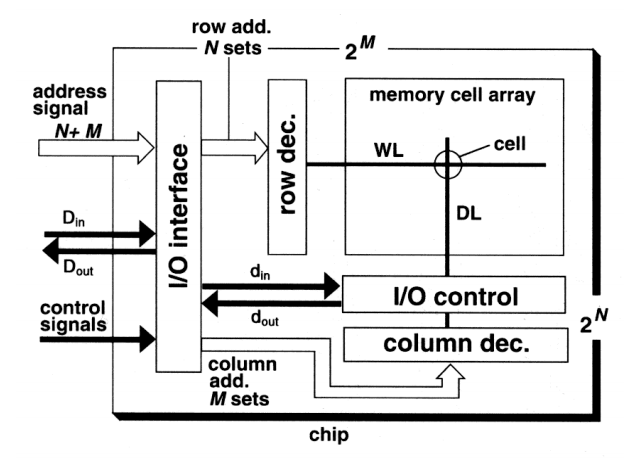
\includegraphics[width=\textwidth]{RAM.png}
  \caption{Общая схема памяти на полупроводниковых технологиях описанная в \cite{DRAM-II}}
  \label{pic:ram_array}
  \end{figure}

Массив, содержащий матрицу из $2N$ строк и $2M$ столбцов, может хранить двоичную информацию из $2N + M + K-1$ битов. Каждый элемент может хранить K битов (обычно K = 1). Например, 4-Мбит информации может быть сохранено для $N + M = 22 и K = 1$. Любая ячейка может быть доступна произвольно, с помощью выбора  соответствующей строки и столбца. Массив ячеек памяти также называется матрицей или ядром. Строка называется строкой X или строкой слова, а столбец называется строкой Y, битовой строкой (линией) или строкой данных. Матричное расположение минимизирует количество цепей возбуждения, потому что один драйвер строки слов совместно используется всеми ячейками одной строки, а усилитель считывания - всеми ячейками одного столбца. Периферийная схема соединяет массив памяти и схему интерфейса ввода / вывода, чтобы они могли обмениваться данными друг с другом. Контроллер отправляет данные записи в ячейку памяти в массиве под управлением схемы ввода-вывода. Типичная схема - это декодер. Выбирается логическая схема, соответствующая одной строке или одному столбцу, на основе сигналов адреса из схемы ввода / вывода. Схема ввода / вывода преобразует внешние сигналы, такие как адреса, управляющие такты, сигналы и входы данных, в соответствующие внутренние сигналы, которые активируют периферийную цепь. Кроме того, он выводит данные чтения из массива в качестве вывода данных чипа. При этом буферы ввода и вывода данных и схемы управления тактовыми импульсами также являются типичными компонентами схемы интерфейса ввода / вывода для разгрузки управляющей схемы.


\subsection{Обзор и принцип работы динамической памяти (DRAM) }
\label{sec:dram}
Принцип работы FeRAM очень похож на принцип работы DRAM, поскольку обе памяти основаны на памяти заряда, то есть информация хранится в конденсаторах. Их ячейки памяти также имеют одинаковую конфигурацию: последовательное соединение одного транзистора и одного конденсатора (1T1C). Единственное отличие состоит в том, что элементом хранения, используемым в FeRAM, является сегнетоэлектрический конденсатор. Он физически отличается от диэлектрического конденсатора путем замены диэлектрика, сегнетоэлектрическим материалом. Кроме того, архитектура памяти современных FeRAM была в значительной степени получена из DRAM. Многие популярные схемы, используемые для DRAM, можно найти и в FeRAM. В следующем разделе описаны принципы работы и базовая архитектура DRAM, а также основные схемы.


На рисунке \eqref{DRAMsc} показан концептуальный массив из одной ячейки  и фактическая конфигурация линии данных и усилитель чтения с защелкой (SA). Усилитель подключаются к каждой паре линий данных (DL), именуемой так же битовая линия(BL), которые обмениваются данными с парой общих линий ввода / вывода данных. С 1-T ячейкой  проводяться операции чтения, записи и обновления. Все операции влекут за собой общие операции: предварительная зарядка всей линий передачи данных к плавающему  напряжению $V_{dd}/2 $ путем включения и выключение схемы предварительной зарядки, а затем активации выбранного слова строки.

\begin{figure}
  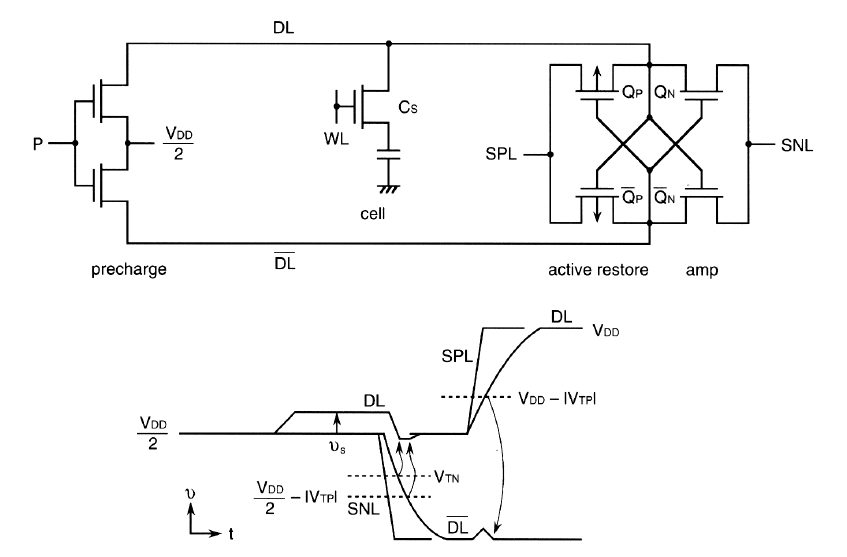
\includegraphics[width=\linewidth]{DRAM-sc.png}
  \caption{Простейшая схема устройства DRAM ячейки, доступа к ней и усилителя чтения \cite{DRAM-II}.}
  \label{DRAMsc}
\end{figure}


Для записи единицы конденсатор ячейки памяти заряжается через транзистор  до $V_{dd} $ , для записи нуля же до $V_{ss}$. Последующее чтение происходит следующим образом: DL заряжается до напряжения $\frac{V_{dd}}{2} $ , после этого открывается транзистор ячейки, и далее напряжение на DL становиться равным $\pm V_s$, если же емкость ячейки есть $C_s$, а емкость Битлайна $C_D$, то выражение для напряжения на линии данных запишется как:
 $$\pm V_s =\frac{V_{dd}}{2}\frac{C_s}{C_s+C_d}  $$
 Где знак зависит от того как была заряжена ячейка перед чтением.


К сожалению,$V_s$  по своей природе мал (100-200 мВ), потому что паразитная емкость $C_D$ линии данных намного больше, чем накопительная емкость $C_s$ ячейки. Небольшой $C_s$ и большой $C_D$ возникают из-за необходимости иметь малый размер ячеек и подключения большого их количества на линии данных соответственно. Следовательно, исходный большой компонент сигнала ($\frac{V_{dd}}{2} $, обычно 1,0-2,5 В) в узле хранения падает до $V_s$. Чтение производится соотстветвующим каждой отдельной битовой линии усилителем.  Характеристики деструктивного считывания (DRO) требуют последовательного усиления и восстановления для каждой из ячеек вдоль строки слова. Это выполняется параллельно с помощью дифференциального чувствительного усилителя  с защелкой на каждой линии данных, а другая линия данных (DLB) используется в качестве эталона. Затем один из усиленных сигналов выводится в виде дифференциального напряжения на линии ввода / вывода путем активации выбранной линии столбца, YL.
Операция записи всегда сопровождается предшествующей операцией чтения. После почти полного завершения вышеупомянутого усиления набор дифференциальных напряжений данных VDD и 0 В вводится из линий ввода / вывода в выбранную пару линий данных. Следовательно, старые данные ячейки заменяются новыми данными. Следует отметить, что вышеописанная операция чтения (то есть усиление и восстановление) выполняется одновременно для каждой из оставшихся ячеек в выбранной строке слов, чтобы избежать потери информации.
Сохраненное напряжение каждой ячейки, ухудшенное током утечки, восстанавливается операцией повторного обновления, которая почти такая же, как и для операции чтения, за исключением того, что все YL остаются неактивными. Это делается путем чтения данных ячеек в строке слова и восстановления их для каждой строки слова, чтобы все ячейки сохраняли данные, по крайней мере, для tREFmax. Здесь tREFmax - это максимальное время обновления для соты. Таким образом, каждая ячейка периодически обновляется с интервалами tREFmax, хотя каждая ячейка обычно имеет время хранения данных, намного большее, чем tREFmax.
Основные проблемы проектирования схемы 1-T соты можно суммировать как отношение сигнал / шум (S/N), рассеяние мощности и скорость из-за следующих присущих характеристик соты \cite{DRAM-I}
\begin{enumerate}
	\item Небольшой сигнал чтения и относительно большой уровень шума. Таким образом, операция чтения является нестабильной, пока не будет достигнут высокий уровень отношения сигнал / шум ( S / N ). Небольшой сигнал чтения вызван тем, что ячейка не имеет усиления. Во время операции чтения существует много источников шума:
	
	\item Конструкция усилителя
	\begin{itemize}
	
	
		\item Трудность размещения усилителя считывания и схемы предварительного заряда в пределах небольшого шага разметки линий данных приводит к возникновению электрического дисбаланса на паре линий данных.
		\item Большое количество усилителей считывания приводит к большому разбросу порогового напряжения (напряжения смещения) между парами транзисторов в усилителе считывания.
		\item Одновременная зарядка и разрядка многих  линий большой ёмкости с высоким напряжением неизменно создают много видов шума.
		\item Кроме того, токи утечки элементов и попадания альфа-частиц, которые ухудшают накопленные заряды, эффективно работают как шумы.
	\end{itemize}
\item Замедленная работа усилителя. Относительно плохая управляемость усилителя считывания, обусловленная необходимостью небольшой площади и работой на основе низкого напряжения на половинном VDD, делает работу усилителя считывания медленной. Таким образом, время считывания является самой большой составляющей времени доступа для чипа.
\end{enumerate}






\section{Обзор динамической сегнетоэлектрической памяти (FRAM)}

\label{sec:fram}


\subsection{Понятие сегнетолектрика и сегнетоэлектрического конденсатора}
\label{subsec:ferro}
В физике сегнетоэлектрик -- это материал обладающий перманентной поляризацией, причем таких состояний у него два, и он способен переходить из одного в другое под действием  электрического поля. Где поляризацию можно считать дипольным моментом системы.

$$ \vec{P} = \sum_{j}Q_j\vec{R_j}   $$

Явление сегнетоэлектричества аналогично явлению ферромагнетизма и в англоязычной литературе носит название ферроэлектричества (англ. ferroelectricity). 


В качесте устройства же мы будем рассматривать сегнетоэлектрический конденсатор (ferroelectric capacitor), который представляет из себя конденсатор вместо диэлектрика у которого используется сегнетоэлектрик. Такой элемент будет напоминать своим поведением конденсатор, однако обладать перманентной спонтанной поляризацией, которую возможно изменять прикладывая напряжение к обкладкам, в частности если напряжение выше коэрцессивного, то поляризация меняет знак, а по цепи протекает ток, перераспределяя заряд на обкладках.

\begin{figure}
  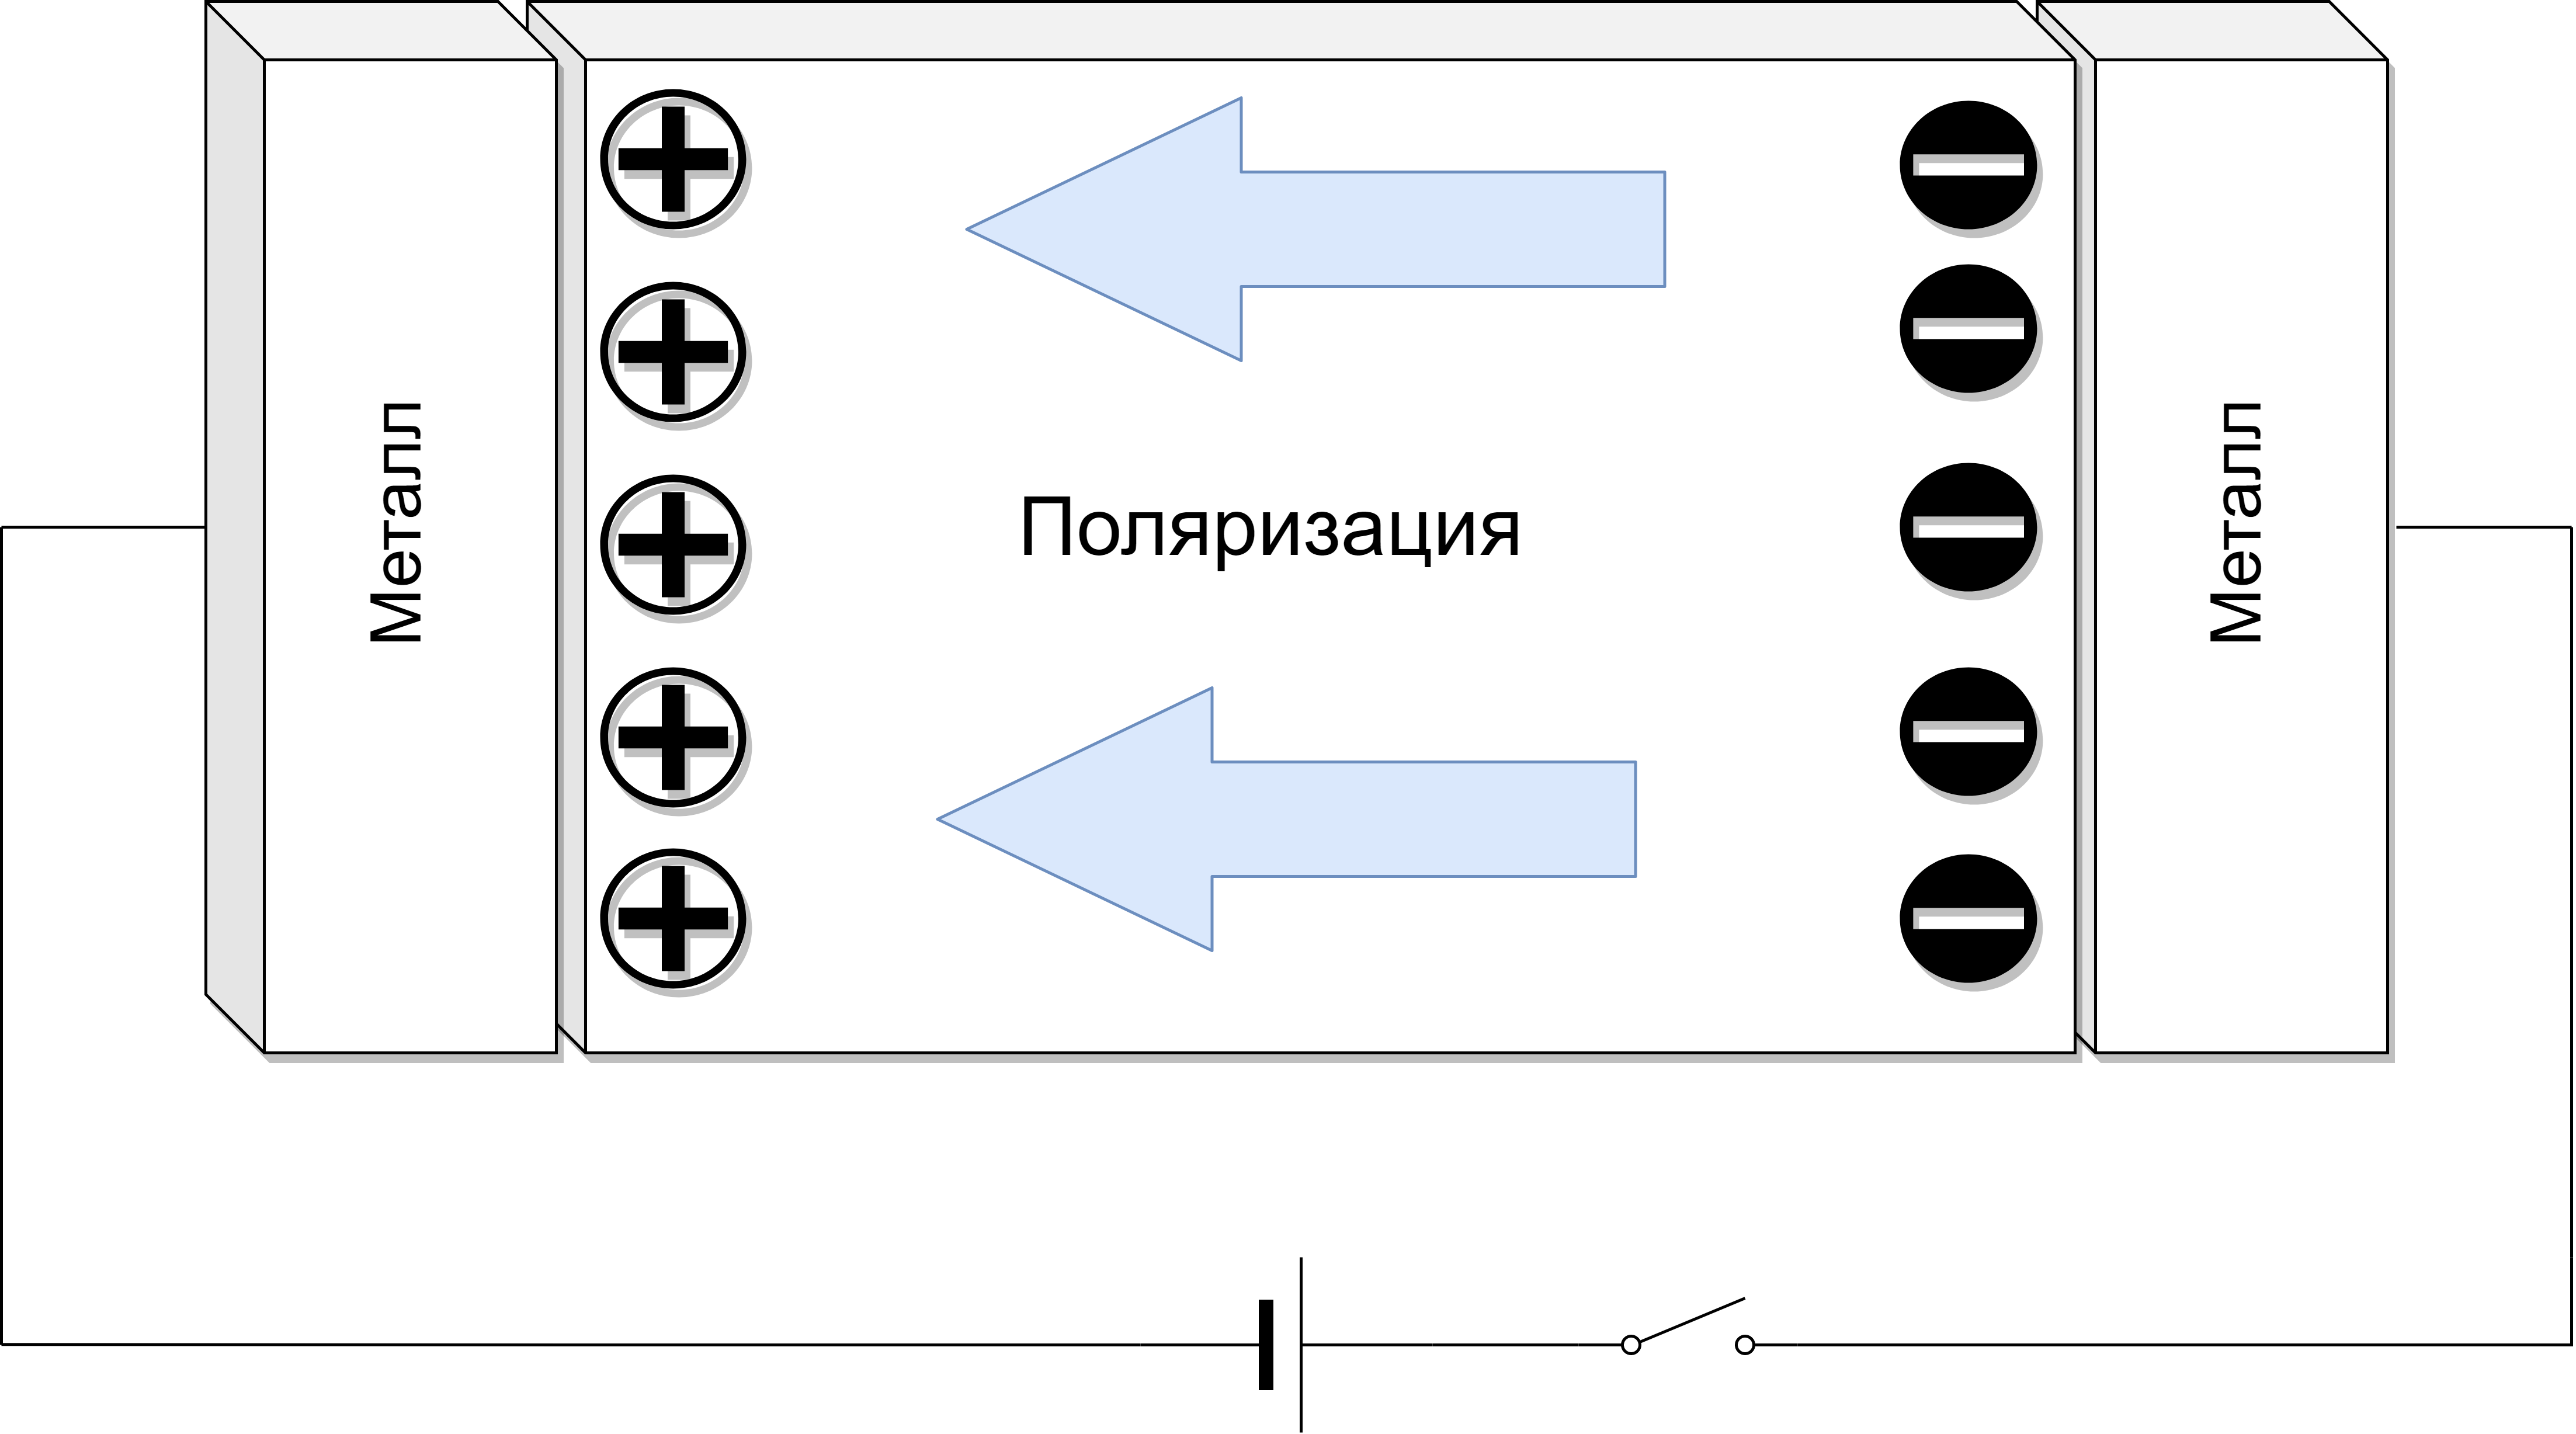
\includegraphics[width=\linewidth]{FRAM-Page-4.png}
  \caption{Схема сегнетоэлектрического конденсатора и создание поля в нем.}
  \label{FerroCap}
\end{figure}





\subsection{Материалы пригодные для создания сегнетоэлектрических конденсаторов}


\subsubsection{Предшествующие поколений сегнетоэлектрической памяти}\

Два сегнетоэлектрических материала, наиболее перспективных для применения в памяти в начале 2000х, представляли собой цирконат-титанат свинца, $Pb (Zr_x Ti_{1-x}) O_3 \ $ (PZT) и танталит висмута-стронция, слоистый перовскит$ SrBi_2Ta_2O_9 $(SBT). Оба относятся к семейству перовскитных кристаллов. Спонтанная поляризация у перовскитов обусловлена смещением катиона из его центрального положения в середине кислородных октаэдров. Как показано на рисунке \eqref{state-Seqneto}, катион находится в одном из двух стабильных положений, и это положение обратимо под действием электрического поля.







\begin{figure}[H]
  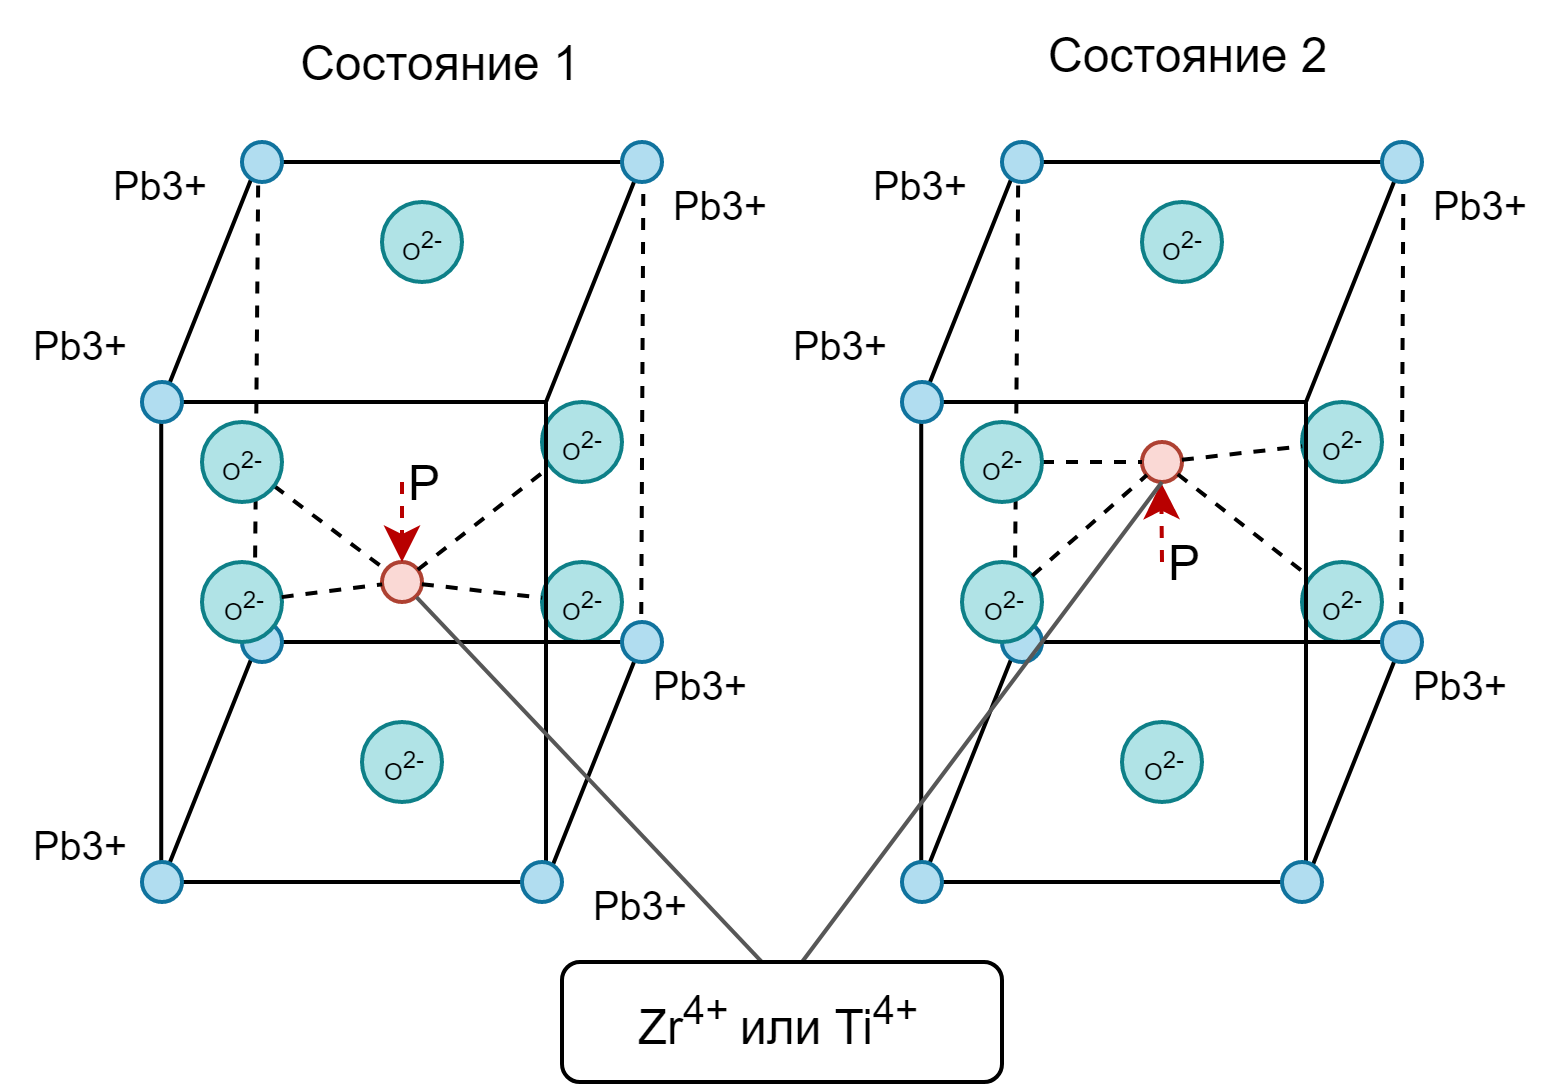
\includegraphics[width=\linewidth]{state-Segneto.png}
  \caption{Перовскитная структура тетрагонального $Pb (Zr_x Ti_{1-x}) O_3 \ $ (PZT) }
  \label{state-Seqneto}
\end{figure}




\subsubsection{$Hf_{0.5}Zr_{0.5}O_2$ как перспективный материал производства сегнетоэлектрической памяти нового поколения}

В последние годы исследования High-K диэлектриков привели к активному исследованию материалов на базе оксидов гафния. В частности в 2016 году ряд авторов из лаборатории атомно-слоевого осаждения МФТИ публикуют статью \cite{Segneto_MIPT-I}, в которой демонстрируются свойства многообещающего материала, который может применяться в качестве сегнетоэлектрика как в FeFET технологии так и в динамической памяти на основе сегнетоэлектрика (FRAM). 

\begin{figure}
  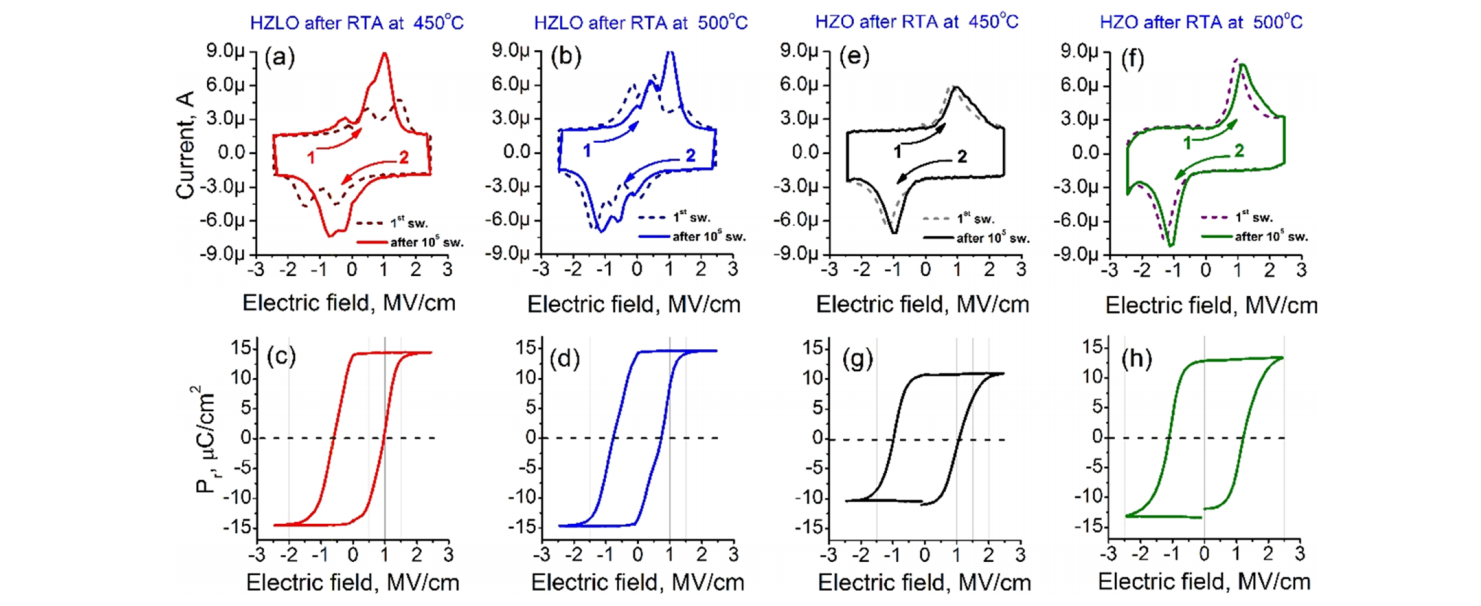
\includegraphics[width=\linewidth]{segneto-graph.png}
  \caption{Графики Поляризации от внешнего поля и ток через элемент при переполяризации, полученные в лабораториях ЦКП в 2016 году \cite{Segneto_MIPT-I} }
  \label{SegDataFig}
\end{figure}

Как видно из рисунка \eqref{SegDataFig} остаточная поляризация таких пленок составила 15 $\mu C/cm^3 $ в течении двух последующих лет путем легирования лантанными примесями удалось улучшить параметры как выносливости материала (количество смены состояния до тех пор пока остаточная поляризация не уменьшится фатально) так и остаточной поляризации. В 2019 году вышла статья \cite{Segneto_MIPT-IV}, где остаточная поляризация достигает уже 30 $\mu C/cm^3 $, при этом выносливость индивидуального конденсатора превышает $ 10^{11} $ циклов \cite{Segneto_MIPT-IV}. Что более чем на 5 порядков больше чем у средней ячейки eFlash памяти. 







\subsection{Ячейки FRAM памяти}
\subsubsection{1T-1C FRAM ячейка}

Принципиальный вид ячейки 1T-1C сегнетоэлектрической памяти представлен на рисунке \eqref{FRAM_fig1}. Как видно он немногим отличается от ячейки DRAM описанной в главе ~\ref{sec:dram} настоящей работы, диэлектрический конденсатор попросту заменяется сегнетоэлектрическим, а второй вывод конденсатора подключается не к земле, а к драйверу PL (plate  line). Таким образом Ячейка сегнетоэлектрической памяти состоит из транзистора доступа, соединенного последовательно с сегнетоэлектрическим конденсатором ( рис. ~\ref{FRAM_fig1}). Для записи единицы напряжение выше коэрцессивного  прикладывается к ячейке через драйвер присоединенный к линии данных (BL) ,  а запись нуля прикладывая напряжение к контакту PL, при этом сегнетоэлектрик в конденсаторе переходит в одно из двух состояний. При этом как наглядно видно из графика \eqref{SegDataFig}, при этом через конденсатор протекает ток, связанный с зарядом который перетекает при перемене поляризации. Таким образом ток протекает через конденсатор в одну сторону если он переходит из состояния <<1>> в <<0>> или из <<0>> в <<1>>, но не протекает если состояние не меняется. 

\begin{wrapfigure}{r}{0.5\textwidth}
  \begin{center}
    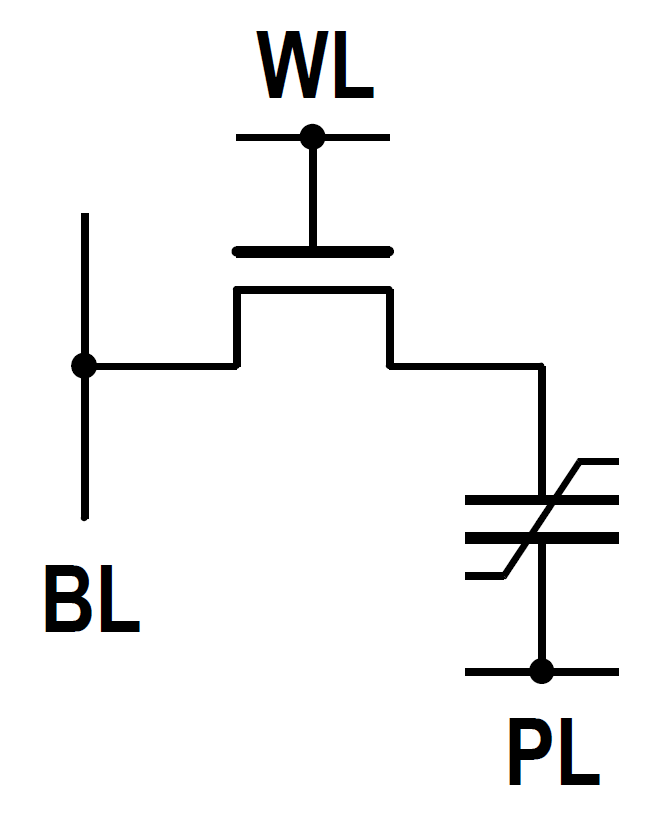
\includegraphics[width=0.48\linewidth]{FRAM-fig1.png}
  \end{center}
  \caption{1T1C Ячейка FRAM }
  \label{FRAM_fig1}
\end{wrapfigure}


\subsubsection{2T-2C FRAM ячейка}

Ячейка 2T-2C состоит из двух ячеек 1T-1C, которые имеют общую линию доступа (WL)  и общий плейт лайн (PL), но соединены с двумя отдельными битовыми линиями (рисунок \ref{pic:2t2c}). Эта ячейка памяти не требует референсного напряжения, потому что она хранит как данные, так и дополнение данных. Для чтения заряда обоих сегнетоэлектрических конденсаторов одновременно сбрасывается на битовую линию и разрядную линию (BLB), а усилитель читения  выполняет дифференциальное сравнение напряжений на битовой и  разрядной линиях. Эта ячейка памяти менее восприимчива к помехам, вызванным производственными изменениями и усталостью материала, так как такие изменения имеют тенденцию оказывать дополнительное влияние на сохраненную поляризацию.

   \begin{figure}[H]
  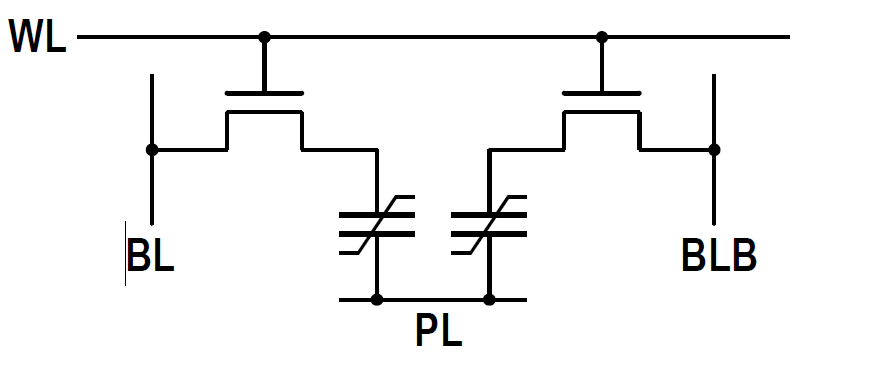
\includegraphics[width=0.7\textwidth]{2T-2C.png}
  
  \caption{Схема ячейки 2T-2C }
  \label{pic:2t2c}
  \end{figure}

\subsubsection{CFRAM ячейка}

Так же существует вид CFRAM ячейки.
Для  улучшения плотности и скорости, была разработана  сегнетоэлектрическая память цепного типа (CFRAM)
было предложено \cite{CFRAM}. В отличие от обычного FeRAM, транзистор и конденсатор ячейки CFRAM соединены параллельно, а не последовательно (рис. \ref{pic:CFRAM_cell}). Отдельные ячейки затем выстраиваются в цепочку (рисунок  \ref{pic:CFRAM}), обеспечивая очень компактную компоновку
(разделение диффузионных областей), таким образом уменьшая среднюю площадь на бит по сравнению с обычным FeRAM. Поскольку размер ячейки является ключевым параметром для полупроводниковой памяти, CFRAM кажется ведущим кандидатом на FeRAM высокой плотности.

\begin{figure}
  \begin{subfigure}[b]{0.3\textwidth}
    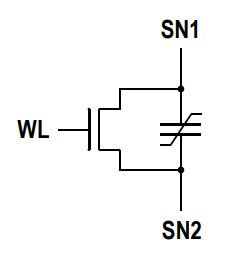
\includegraphics[width=\textwidth]{CFRAM_cell.png}
    \caption{Индивидуальная CFRAM ячейка)}
    \label{pic:CFRAM_cell}
  \end{subfigure}
  %
  \begin{subfigure}[b]{0.7\textwidth}
    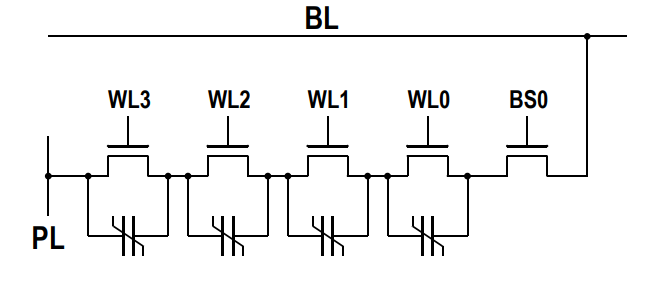
\includegraphics[width=\textwidth]{CFRAM.png}
    \caption{Массив CFRAM памяти}
    \label{pic:CFRAM}
  \end{subfigure}
  \caption{Конструкция CFRAM памяти.}
\end{figure}


\subsubsection{Необходимый размер ячейки}
Определение конденсатора подходящего размера  для заданного количества ячеек на битовую линию или наоборот, не является тривиальным для FeRAM. В отличие от DRAM, увеличение размера конденсатора ячейки не всегда приводит к увеличению напряжения сигнала. Это связано с тем, что во время считывания напряжение на плейт линии (например, $V_{PL} $) распределяется в соответствии с делителем конденсатора, который образован конденсатором ячейки и паразитной емкостью CBL разрядной линии (см. ). Чтобы переключить поляризацию внутри сегнетоэлектрика, напряжение на сегнетоэлектрическом конденсаторе $V_{pl}$ должно превышать коэрцитивное напряжение $V_c $, следовательно,$ V_{pl} \geqslant V_C$. Это обстоятельство накладывает первое требование на емкость разрядной линии, которая выполняется, если выполняется следующее соотношение:

\begin{equation}
	V_{pl} \geqslant V_C  \Rightarrow C_{BL} \geqslant \frac{V_c C_s}{V_{PL} - V_c}  
\end{equation}


На практике вышеприведенное уравнение представляет только минимальное требование, и обычно VFE = VC недостаточно. Как правило, напряжение на конденсаторе - после того, как конденсатор сбросил свой остаточный заряд $Q_r $  на битовую линию - должно быть в два раза больше его коэрцитивного напряжения, чтобы привести сегнетоэлектрик к полному насыщению \cite{fram18}. В противном случае напряжение сигнала будет слишком маленьким. Следовательно, более строгие требования к CBL:


$$ C_{BL} \geqslant \frac{2Q_r + 2V_c C_s }{V_{PL} - V_c  }  $$



  \begin{figure}[H]
  \centering
  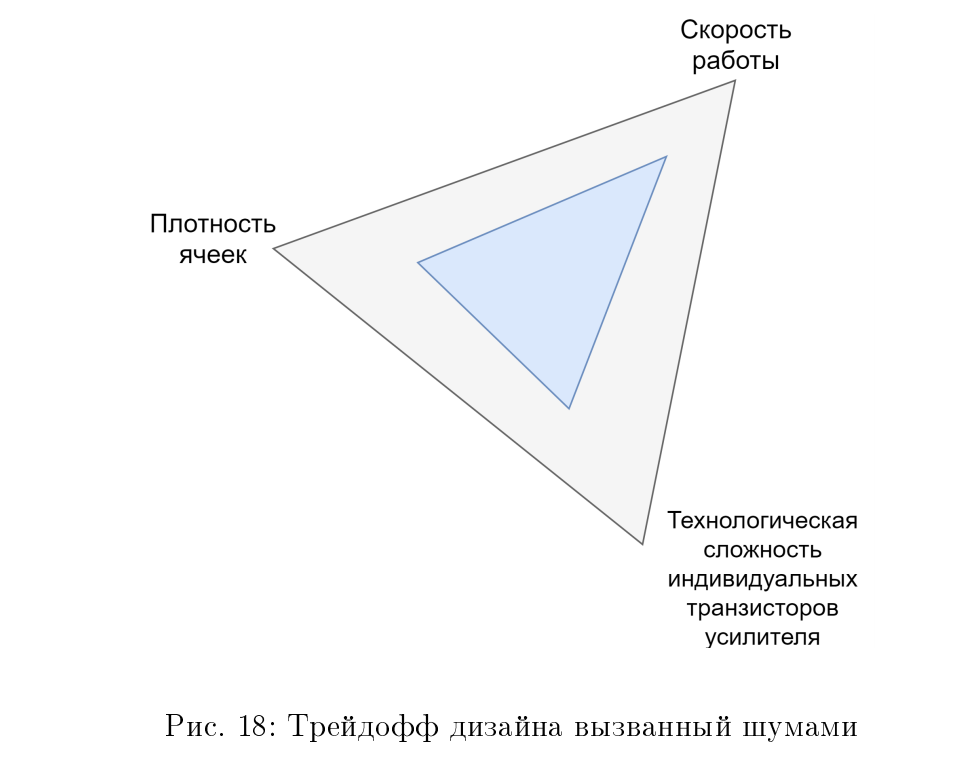
\includegraphics[width=0.6\textwidth]{19.png}
  \caption{Зависимость считываемого сигнала в зависимости от ёмкости битлайна из \cite{lib:c_bl}}
  \label{pic:19}
  \end{figure}


\subsection{Схема устройства и операции FRAM памяти}

Из-за множества аналогий между DRAM и FeRAM, некоторые проблемы проектирования FeRAM уже известны из DRAM и были решены путем применения предыдущих решений DRAM. Тем не менее, есть также ряд проблем, которые являются уникальными для FeRAM. Из этих десяти проблем критические проблемы проектирования, требующие инновационных решений. В этой главе представлены некоторые из наиболее актуальных вопросов, затрагивающих настоящие и будущие FeRAM.





Существует несколько компановок FRAM, но все они похожи по своему устройству. Рассмотрим две базовые из них:
\subsubsection{1T-1C FRAM компановка}
Наиболее подробно в данном обзоре я остановлюсь именно на обзоре памяти на 1T-1C ячейках, имо именно она была использована в нашей работе при разработке тестового чипа (глава \ref{sec:test_chip}). 



   \begin{figure}[H]
  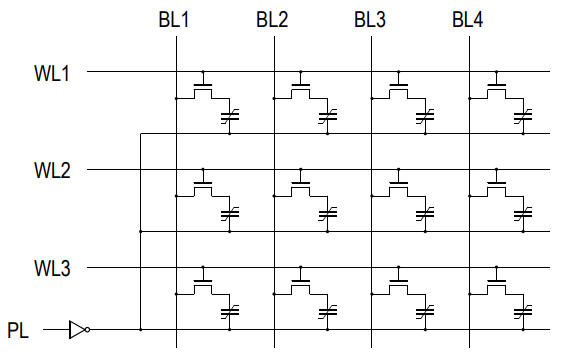
\includegraphics[width=\textwidth]{FRAM_array.png}
  \caption{Схема массива 1T-1C fram памяти}
  \label{pic:fram_array}
  \end{figure}







\subsubsection{Операция записи}
1T-1C ячейки компануются в массивы представленный на рисунке \ref{pic:fram_array} 



Для записи в выбранную ячейку массива, в битовой линии N и строке доступа M ($WL_M$), активируется соответствующая WL строка, открывая транзистор доступа к ячейке, далее активируется либо драйвер нужной битовой линии поднимая ее до высокого напряжения, если требуется записать <<1>>, или соответствующий драйвер плейт линии ($PL_N$) если нужно записать <<0>>. После чего ячейка  переходит в соответствующее состояние, и память готова к следующей операции.

\subsubsection{Операция чтения}
Операция чтения по своей сути сложнее операции записи и занимает больше тактов работы памяти. Для чтения выбранной ячейки в битовой линии N и строке доступа M ($WL_M$), активируется соответствующая WL строка, при этом битовая линия остается изолированной от земли, и драйвер напряжения битовой линии отключается от питания, таким образом битовая линия превращается в конденсатор. После чего происходит операция сходная с записью нуля в ячейку памяти: поднимается напряжение на соответствующем плейт лайне ($PL_N$). После чего, если ячейка была в состоянии <<1>> то при переполяризации заряд остаточной поляризации $Q_r$, перетечет на битлайн, если ячейка и так была в этом состоянии (записан ноль) то переполяризации не произойдет, и битлайн останется в околонулевом состоянии. На рисунке \ref{pic:bl_read} представлены данные Симуляции вольтажа битовой линии при последовательных операциях записи <<1>>, чтения <<1>>, чтения <<0>>, тестового чипа описанного в пункте \ref{sec:test_chip}, при емкости битлайна  $C_{BL}=500pF $ и емкости ячейки $~10^{-13} С $ в среде Cadence virtuoso. Как видно заряд стекающий при переполяризации как правило мал по сравнению с $V_{dd} $, в данном случае  $V_{dd}=2.5V $, причем как было описано в секции \ref{sec:dram}, напряжение $$ \Delta V = \frac{Q_r}{C_{BL}}   $$ зависит как от емкости ячейки, так и от размеров битлайна. Таким образом, чем больше битлайн (как следствие общее количество ячеек) тем меньшую разность  напряжений $ \delta V $ мы будем фиксировать при чтении, то же самое будет происходить при уменьшении размеров сегнетоэлектрических конденсаторов, будет уменьшаться читаемый заряд. Размер читаемого заряда будем определять возможность работы памяти, так как шумовые характеристики усилителя чтения описанные в пункте \ref{sec:noise} настоящей работы, будут определять возможность работы прибора как памяти. Усилителю << Проще >> безошибочно прочитать большую разность зарядов. Соответственно скорость работы и размер ячеек при дизайне конкретного чипа будут зависить от ожидаемых  шумовых характеристик усилителя чтения, который далее попросту сравнивает это напряжение с некоторым лежащим между $ V_{ss}= 0  $ и $ V_{+}= V_{ss} + \Delta V   $. После сравнения уже усилитель возвращает в цифровую логику сигнал уровня $V_{ss}  $ или $V_{dd}  $ , соответствующий нулю или единице.

   \begin{figure}[H]
  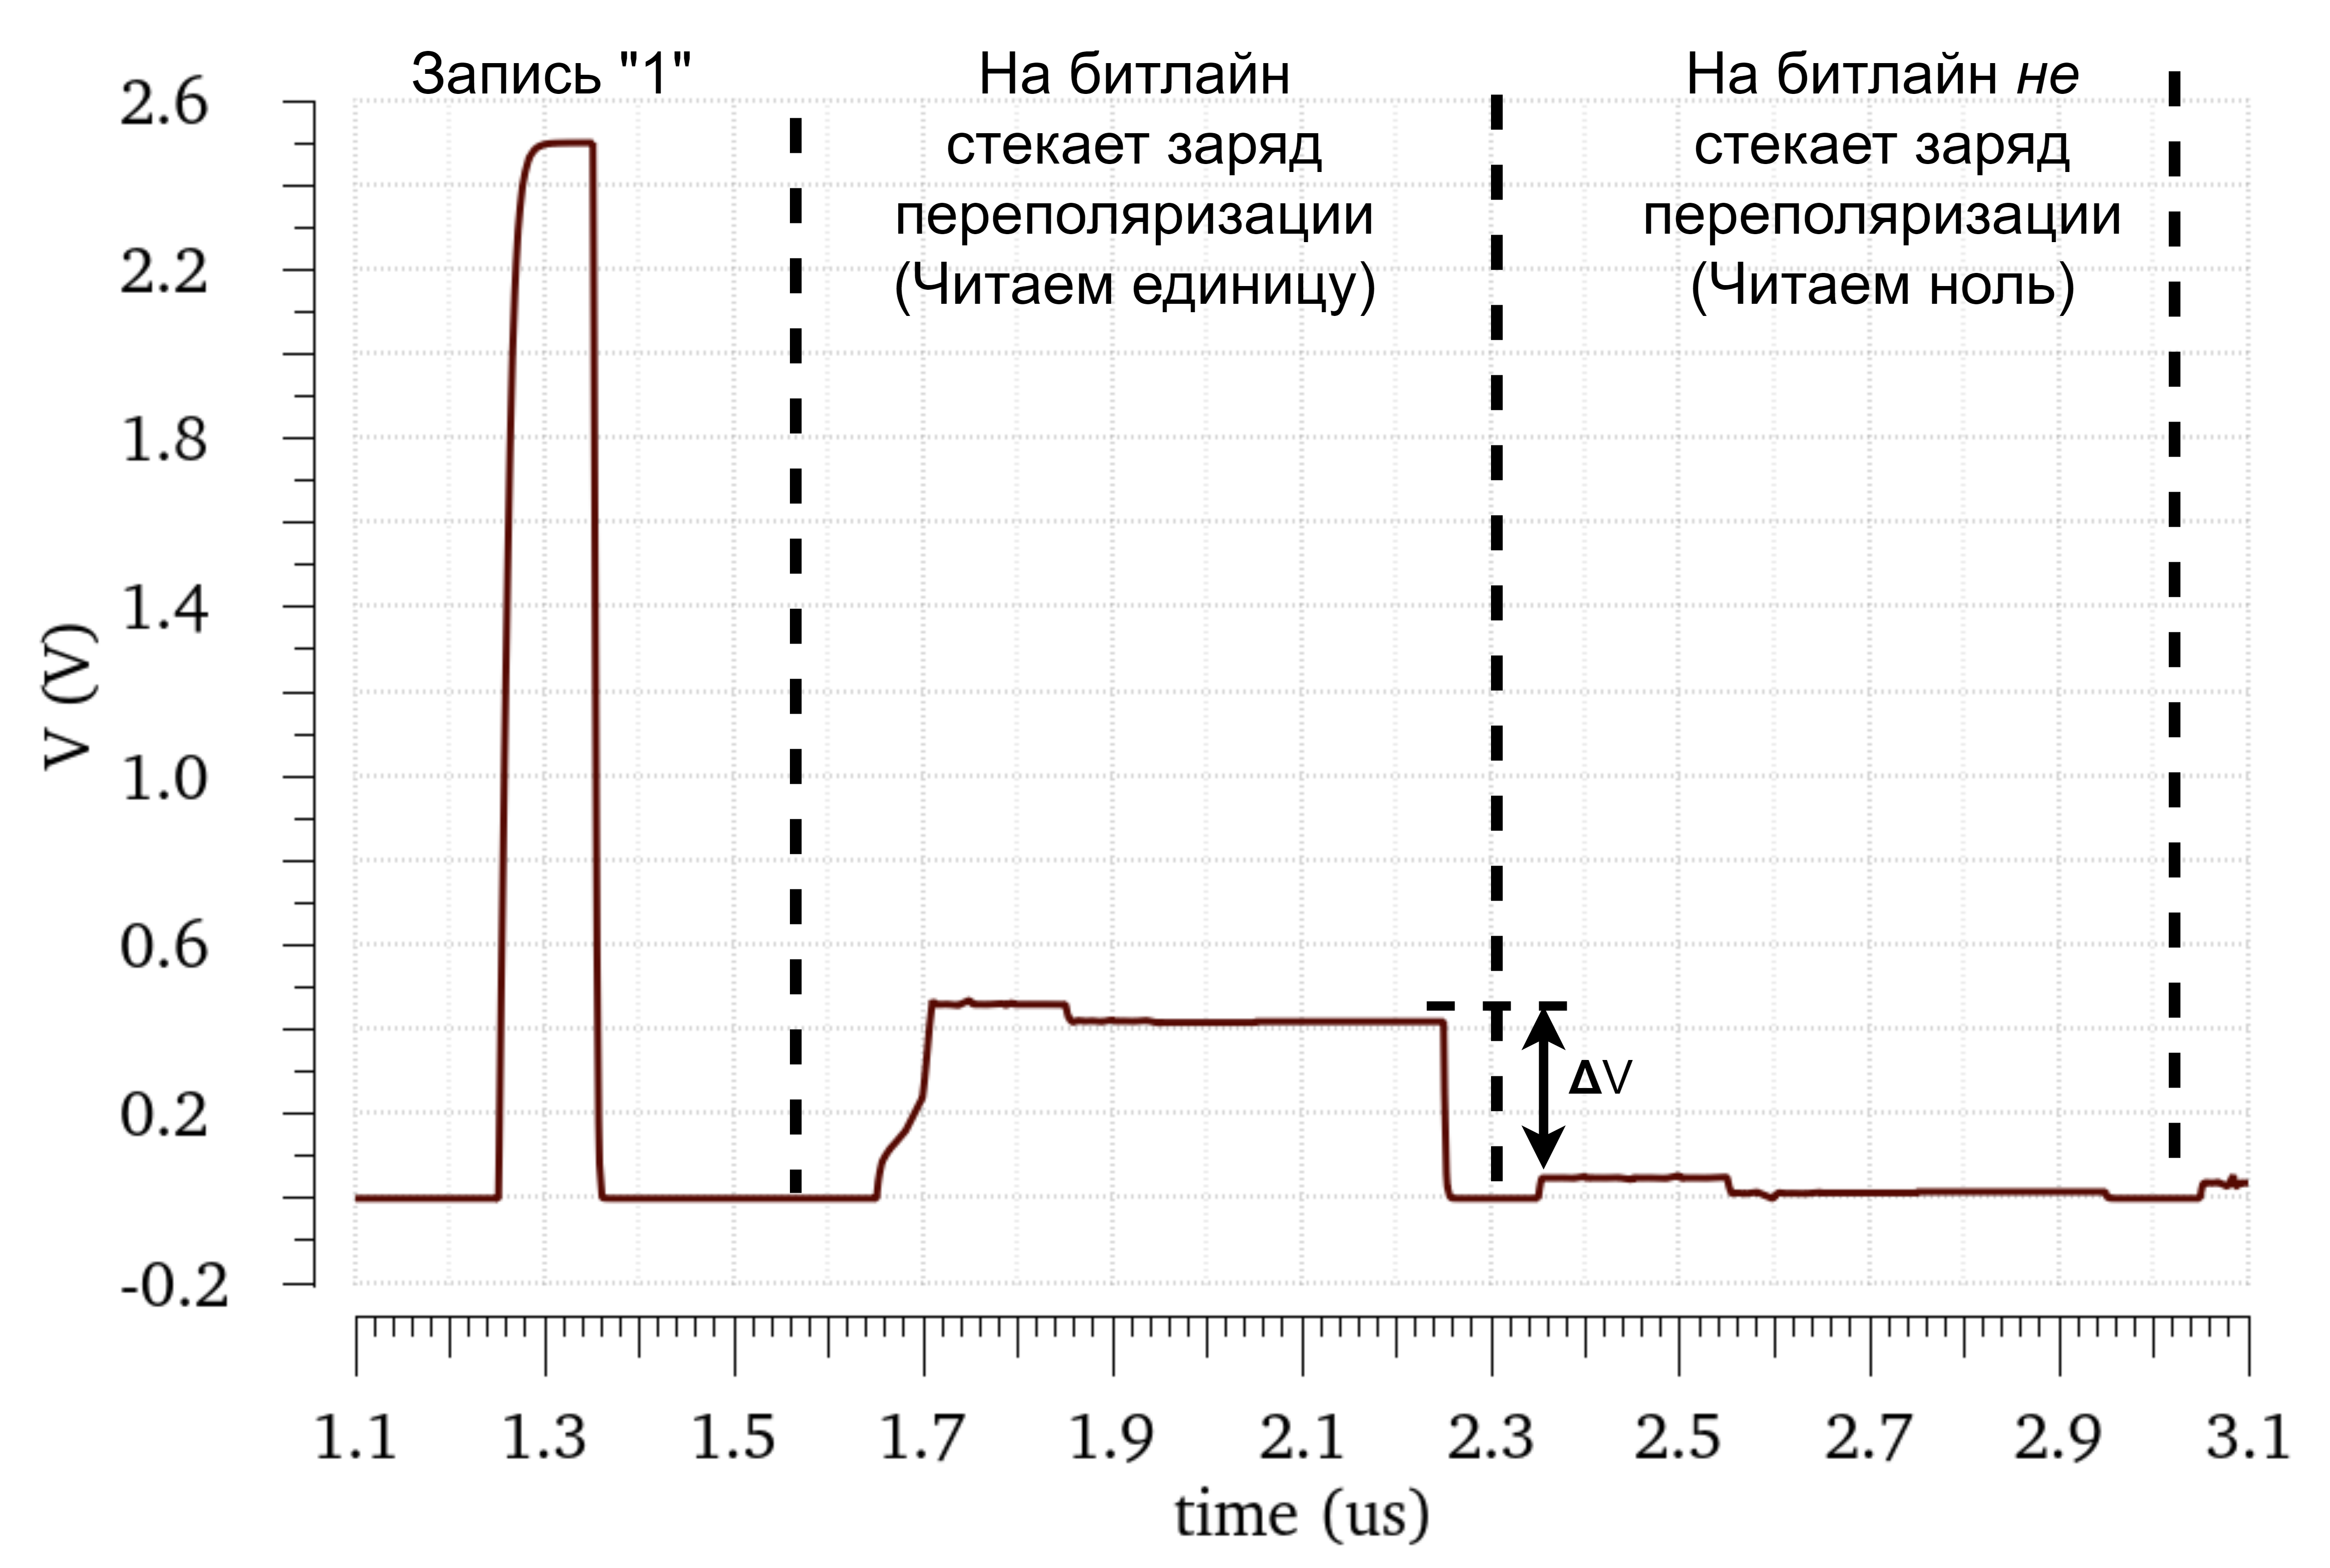
\includegraphics[width=\textwidth]{FRAM-BL.png}
  \caption{Симуляция вольтажа битовой линии при последовательных операциях записи <<1>>, чтения <<1>>, чтения <<0>>, тестового чипа описанного в пункте \ref{sec:test_chip}, при емкости битлайна  $C_{BL}=500pF $ и емкости ячейки $~10^{-13} С $ в среде Cadence virtuoso }
  \label{pic:bl_read}
  \end{figure}



\subsubsection{Преимущество и недостатки}
Преимущество этой архитектуры состоит в том, что один драйвер задействован для работы с одной линией поэтому эффективность области может быть относительно   высокой. Недостатком является то, что в любое время есть один активный ряд и большое количество неактивных строк, которые, тем не менее, вносят вклад в общюю емкостную нагрузку. В результате высокая емкостная нагрузка замедляет рост и спад напряжения  плейт лайна. Таким образом, скорость FeRAM замедляется соответственно.












\section{Разработка тестового чипа}
\label{sec:test_chip}

\subsection{Описание процесса реализации разработки}

Что же есть процесс разработки интегральной схемы памяти? В этой главе мы ответим на вопрос как  была проведена разработка. Первым делом нужно заметить что сам кристалл делиться на аналогувую и цифровую часть. Цифровая часть отвечает за связь с компьютером эксплуатирующим память, а так же за подачу управляющих сигналов. 
Аналоговая же часть в свою очередь, отвечает за саму структуру памяти, а так же за цифро аналоговое и аналого-цифровое преобразование. Разработка цифровой части описана подробно в части \ref{subsec:digital}. И была проведена путем написания кода verylog, который после этого может как быть использован для симуляции управления чипом, так и для синтеза из него набора транзисторов который будет вести себя в точности как написанный код. Для первоначальной отсладки была использована открытая версия компилятора кода verylog: ModelSim intel FPGA starter edition 18.1 . Аналоговая часть делиться на два важных этапа разработки. Первый это описать поведение распространенных элементов использованных в дизайне: конденсаторов, резисторов ну и конечно транзисторов. Их  поведение описывается многоцелевым симулятором SPICE. Спайс модели компонентов используемых в проектировании аналоговой части чипа содердаться в так называемом PDK (Process design kit) техпроцесса использованного для разработки (см. \ref{subsec:DK}). Первоначальные же прогоны были выполнены в программе Tanner TSpice. Там необходимо было отладить работу аналоговых компонентов, а так же аналогового компонента симуляция которого не существует в SPICE изначально или с PDK, это сеннетоэлектрический конденсатор. Для того чтобы симулировать его поведение был написан код на языке Verylog A, который позволяет проводить аналоговую симуляцию компонента в SPICE задавая его математические параметры. Подробнее о том какая была использована  математическая модель можно почитать в этой главе: \ref{subsec:va}). После чего вся схематика была переведена в САПР среду Cadence Virtuoso, где был получен анализ оптимизации (см. \ref{sec:analisis} ). Только после этого в Virtuoso, используя TSMC 65nm PDK было начато проектирование layout. Результаты которого можно посмотреть в приложении (\ref{pic:array_la}) , и в соответствующей главе (\ref{sec:layout}).

\subsection{Разработка достоверной симуляции поведения сегнетоэлекторического конденсатора}
\label{subsec:va}
В данной секции работы мы рассмотрим базовые представления о физике сенетоэлектрика, в отрыве от его приложения, и построим модель необходимую для его симуляции при разработке памяти.




Чтобы построить способ симулировать модель сегнетоэлектрического конденсатора описанного в главе ~\ref{subsec:ferro}, перейдем к краткому рассмотрению теории фазовых переходов Ландау, которая описывает состояние ферромагнетиков и сегнетоэлектриков. В дальнейшем  $\mathcal{F} $ есть свободная энергия, а $ \vec{P}$ есть параметр порядка   .\\
  Тогда справедливо выражение:
  \begin{equation}\label{fermi}
   \mathcal{F} = \frac{1}{2}\alpha \vec{P}^2 + \frac{1}{4}\beta \vec{P}^4 - \vec{E}\vec{P}
  \end{equation}
 Где $ -EP  $ есть энергия внешнего электрического поля: с напряженностью E, находим ее из напряжения, зная толщину сегнетоэлектрика $U= \vec{E}d $. У этого графика при $E=0 $ есть два локальных минимума и один локальный максимум, локальные минимумы представляют собой устойчевые состояния системы (те самые два состояние яегнетоэлектрика), а локальный максимум неустойчевое состояние. Зависимость $\mathcal{F}(\vec{P})$ в общем виде представленана рисунке \ref{pic:f}.
 
 
   \begin{figure}
   \centering
  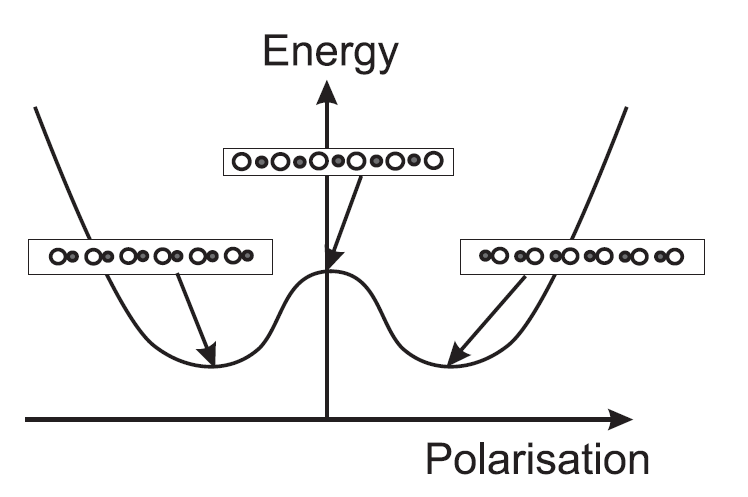
\includegraphics[width=0.8\textwidth]{F(P).png}
  \caption{Примерный график $\mathcal{F}(\vec{P})$ \cite{ferro}}
  \label{pic:f}
  \end{figure}
 
 
 Чуть лучше это можно заметить если перейтик производной энергии. Дифференцируя выражение \eqref{fermi} получаем:
  \begin{equation}\label{dfermi}
  \frac{\partial \mathcal{F}}{\partial P }  = \alpha P + \beta P^3 - E
  \end{equation}
  График выражения \ref{dfermi} представлен на рисунке \ref{pic:diff}.
  
  
  
  
     \begin{figure}[H]
   \centering
  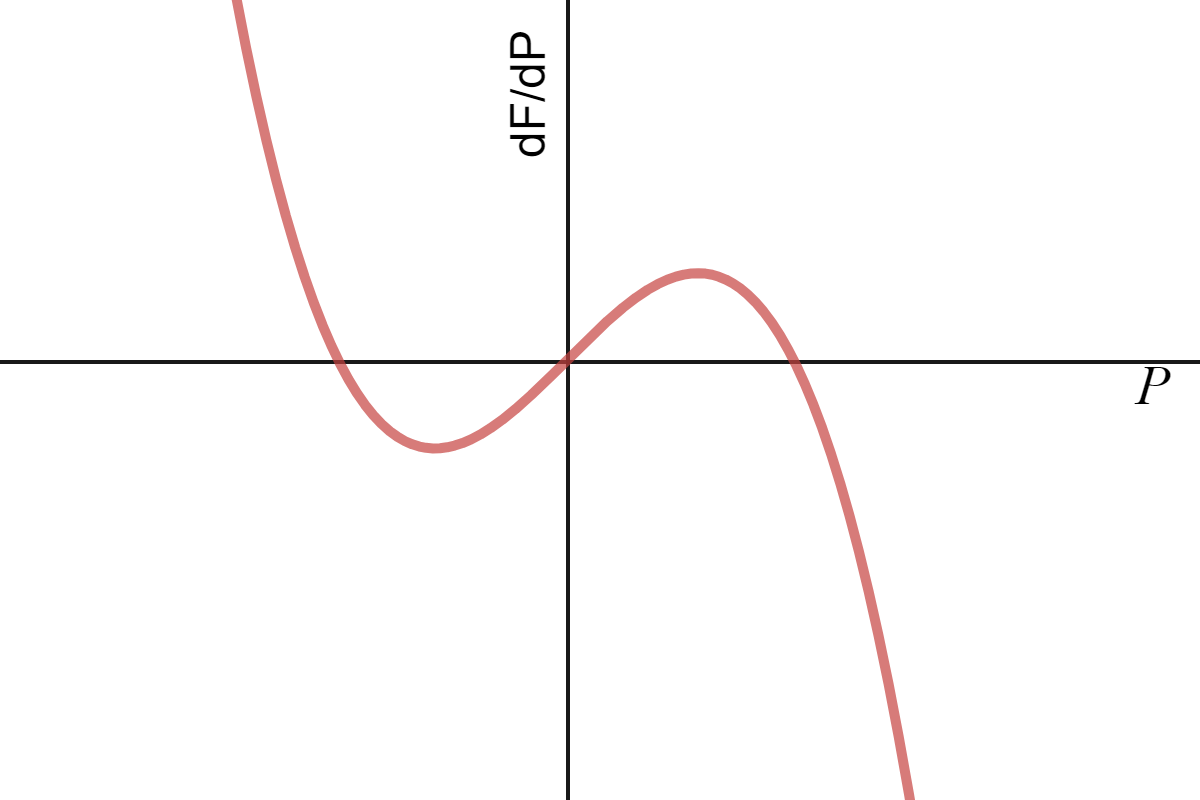
\includegraphics[width=0.8\textwidth]{graph_dgibs.png}
  \caption{Примерный график первой производной энергии при $\vec{E} = 0 $}
  \label{pic:diff}
  \end{figure}
  
   Здесь $E=0 $. Устойчивые состояния представлены точками пересечения функцией оси Х справа и слеваю. Пересечение же в нуле является неустойчивым состоянием (локальнм максимум функции $ \mathcal{F}  $. Приложение же напряжение двигает график вверх и вниз. Заметим, что при движении вверх или вниз при определенном значении $E=E_c $, одно из устойчивых состояний перестанет существовать (график более не будет пересекать ось поляризации). Таким образом если система находилось в этом состоянии то при $E>E_c$ система тут же сместиться в другое состояние. Данная теория называется теорией фазовых переходов Ландау и этот  принцип описывает поведение сверхпроводника, ферромагнетика, сверхтекучей жидкости и сегнетоэлектрика.
   
   
   
   
Это пример фазового перехода второго порядка или непрерывного
где параметр порядка (здесь спонтанная поляризация) обращается в нуль
при температуре перехода $T_c = T_0$. Где $ \alpha = \alpha(T,T_c) $. К счастью для сегнетоэлектриков рассмотренных в главе температура $T_c$ во много раз привосходит комнатную \cite{Segneto_MIPT-I}(стр. D) и колеблятся в пределах $ (300-400) \degree C  $


Для того, чтобы построить гистерезис, нужно найти связь свободной энергии $\mathcal{F} $ с производной поляризации по времени ( чтобы интегрировать/дифференцировать ее).
	 \begin{equation}\label{Rfermi}
		 \frac{\partial  \mathcal{F} }{\partial P} = - R  \frac{\partial  P }{\partial t}  
 	 \end{equation}
 	 Где $ R $ -- аналог сопротивления, есть что-то вроде временной константы, и  выбирается исходя из экспериментально ожидаемого характерного  времени реакции системы.



Осталось связать заданные нами переменные $\alpha $ и   $\beta $ с физичными, измеримыми величинами: $ \vec{E}_c $ и
		  $\vec{P}_0 $ :
		разрешая уравнение второй производной для минимума энергии ( $ \frac{\partial\mathcal{F} }{\partial \vec{P}} $ ) , и пользуясь соотношением (2) для поиска коэрцитивного напряжения, получаем:\\
		$$\alpha = 3\sqrt{3E_c/(8{P_0}^3)}$$\\
	$$ \beta = -3\sqrt{3E_c/(4P_0)}$$\\
	
	
	
	
	  Приравнивая выражение  \eqref{dfermi} к \eqref{Rfermi} получаем :
  
  \begin{equation}
  -R \dot{\vec{P}}  = \alpha \vec{P} + \beta \vec{P}^3 - \vec{E}
  \end{equation}
  Теперь, решая это уравнение относительно заданного нами  $ t $, строим график в виде $P (E(t))$:




\subsection{Дизайн цифрового контроллера и режимы работы чипа}
\label{subsec:digital}

В разработке интегральных микросхем аналогового (Analog) или цифрвого (Digital) типа, приняты две совершенно разные разные парадигмы разработки интеральных схем. Digital разработка подразумевает компиляцию кода на языке verylog в уже готовый layout для CMOS технологии, в ходе так называемого "Синтеза". Соответсвенно парадигма Analog разработки подразумивает размещение топологий отдельных элементов технологии, или даже отдельную конструкцию элементов поскольку нам часто важны с большой точностью их параметры. Соответственно существуют и технологии соединяющие воедино эти две парадигмы, это смешанная симуляция. Она же бывает в свою очередь Analog on top, когда аналоговый блок включается в процесс синтеза в виде отдельного блока с заданными размерами, или же наоборот, когда цифровая часть есть огромный элемент размащаемый при Analog проектировании. В ходе нашей работы рассматривался как Digital on top так и Analog on top поскольку первая выгодна при размещении памяти как отдельного standalone девайса, а вторая при использовании памяти в виде части другого устройства. В этой части работы же я попробую описать способ работы контроллера блока памяти. Сам контроллер представляет из себя явный пример конечного автомата (State Machine) и далее уместно провести примерную схему устройства управляющей части тестового чипа.

\begin{figure}[H]
\centering
  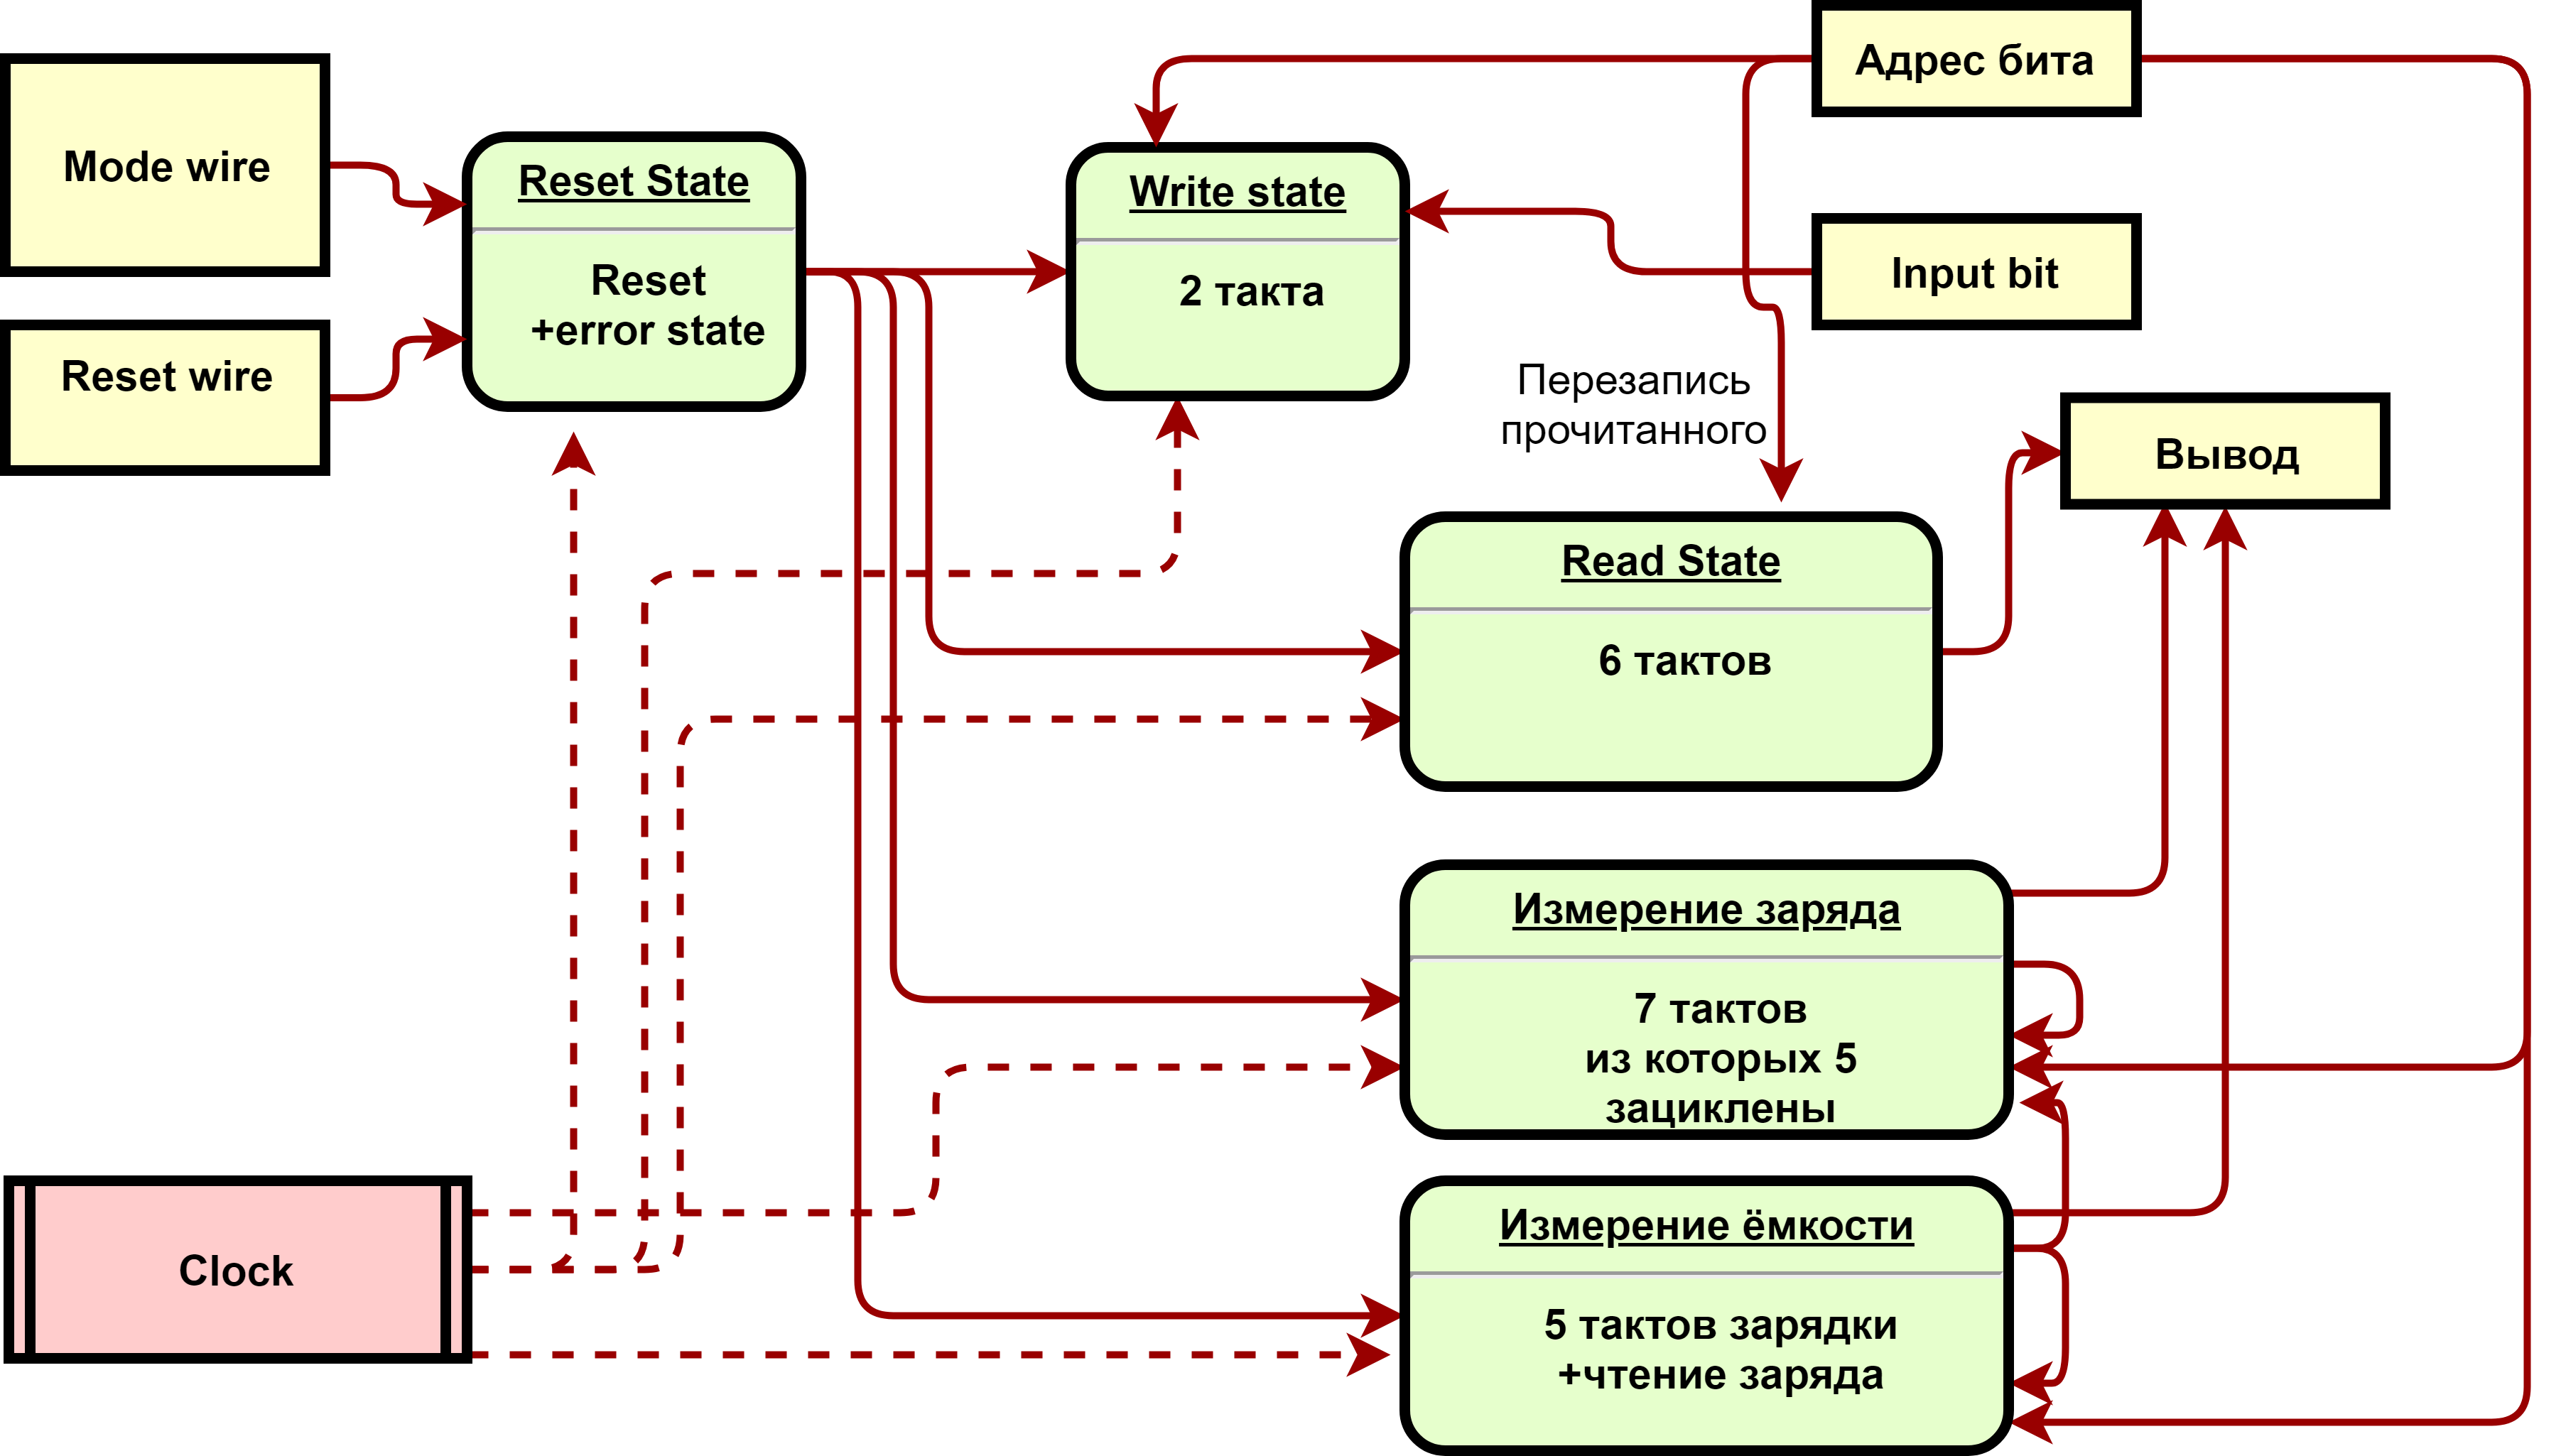
\includegraphics[width=\linewidth]{state.png}
  \caption{Упрощенная схема устройства логической последователности состояний контроллера}%Поправить стрелки от записи к чтению, ДОБАВИТь количество тактов правильное!!!!
  \label{stateFig}
\end{figure}

\subsubsection{Reset}
Согласно схеме у контроллера имеется некое исходное Reset состояние куда машина попадает каждый раз когда поднимается напряжение на Reset, или же каждый раз когда заканчивается одна из операций кроме операции чтения, после операции чтения контроллер переходит в состояние записи прочитанного бита. Итак находясь в состоянии Reset контроллер переводит все внутренние переменные и внешние выводы в некое начальное состояние. Тем самым Reset состояние так же является чем то вроде изначальной параметризации устройства. Далее устройство считывает входное состояние и переходит в него. 




\subsubsection{Запись} Самая короткое по продолжительности состояние, в нем контроллер за 2 такта проводит запись, и уведомляет мастер устройства о том, что запись прошла успешно.

Процесс запипи начинается с того что контроллер получает доступ к конкретной ячейке из массива поднимая напряжение на нужной WL линии массива, и нужном плейт лайне или битлайне ( в зависимости от того нужно ли записать "0" или "1". При этом если напряжение поднимается на PL то пишется ноль, а если BL, то пишется единица. Второй такт нужен чтобы сообщить контроллеру о выполнении операции. 

\subsubsection{Чтение} Операция чтения состоит из 7 тактов. Контроллер открывает WL нужной линии, после чего поднимает напряжение на соответствующем плейт лайне, после чего заряд стекает (или не стекает) либо заряжая битлайн до напряжения  $ V_{BL} \sim 300m  V $, после чего сперва опускает напряжение на плейт лайне и только после этого перекрывает линию WL, тем самым позволяя уйти току который мог уйти на битлайн при переменном напряжении на обкладках конденсатора ячейки. Теперь на битлайне остается либо околонулевое напряжение, либо напряжение $ V_{BL} \sim 300m  V $, которое далее сравнивается с напряжением $ V_{REF_READ} \sim 50m  V $ поданное от генератора референсных сигналов (см. Главу генератор референсных сигналов).
\subsubsection{Точное чтение заряда в ячейке}
\label{subsec:v_scan}
 Фактически операция похожа на обычное чтение, но вместо него используется аналого-цифровое и цифро-аналоговое преобразования чтобы точно определить заряд сброшенный на битлайн. Эта операция является частью диагностики ячеек чипа. В ходе операции заряд сбрасывается на битлайн, далее сравнивается теперь уже не с околонулевым потенциалом а с референсным потенциалом (см. Главу генератор референсных сигналов) далее если результат сравнения дает отрицательный результат (референс меньше) то операция повторяется прибавляя единицу к значению 6-ти битного референсного напряжения (от $ V_{ss}$ до $V_{dd} $) . Таким образом, изменяя его на небольшую величину. При этом же разрешающая способность чипа будет определятсья в первую очередь шумом как описано в секции ~\ref{sec:noise} .
\subsubsection{Чтение емкости}

Этот режим внедрен в чип чтобы с хорошей точностью определить ёмкость каждой битовой линии. Сделано это чтобы убедиться что анализ методом извлечения паразитных параметров ( см. ~\ref{subsec:parasitic})  
дает тот же результат что и фактическая ёмкость битлайна, которая к тому же может отличаться от заданных параметров в виду технологических особенностей, или истоков транзисторов битовой линии в силу charge injection эффекта. Суть метода заключается в том, что на чипе имеются два заранее изготовленных мим конденсатора, с заранее хорошо известной ёмкостью (например $C_1 $ и $C_2 $. Когда требуется провести измерение ёмкости конкретной битовой линии конденсаторы заряжаются до напряжения $V_{dd}$, после чего открывается транзистор доступа одного из конденсаторов к битлайну, заранее предзаряженного до уровня земли. После чего открывется транзистор связывающий битовую линию и тестовый конденсатор и напряжение на них сравнивается. Первоначальный заряд  $ V_{dd}C_1 = Q_1 $ теперь распределен между битовой линией и тестовым конденсатором. То есть теперь система заряжена до некого напряжения $ U $ такого что: $$C_1 U + C_{BL} U = V_{dd}C_1 = Q_1  $$
Теперь остается только изолировать линию и провести точный поиск заряда аналогично предыдущему режиму ( ~\ref{subsec:v_scan} ).



\subsubsection{Поиск напряжение смещения усилителя }



В силу технических неточностей процесса усилитель описанный в части \ref{sec:amp} будет обладать неким напряжением смещения, то есть:

$$ V_{out} = g ( V_{in} - V_{ref} + V_{bias})  $$
,где $V_{bias}$ есть напряжение смещения, и оно может достигать порядка предельной разницы измерения $ \Delta V = V_{in} - V_{ref} $, соответственно хорошей возможностью будет поиск этого смещения путем внедрения соответствующего режима. Определить напряжение смещения легко можно если начать сравнивать два известных заранее сигнала. Таким образом требуется внедрить возможность так же заряжать битлайн от генератора переменных напряжений (см. \ref{sec:r2r}) . 






\subsection{Компоненты чипа}


\subsubsection{Ячейка памяти}

Конечный вид топологии ячейки памяти представлен на рисунке \ref{pic:cell_la}. Между слоями металла размещается слой сегнетоэлектрика, при этом плейт лайн проходит по всем обкладкам верхнего слоя металла. Битовая же линия цепляет исток транзистора доступа и имеет произвольный размер. Линия доступа же при это несколькими переходными отверстиями (см. рис \ref{pic:array_la}) выводится в верхние слои металла и перпендикулярно уходит к цифровой части схемы.

\begin{figure}[H]
  \begin{subfigure}[b]{0.2\textwidth}
    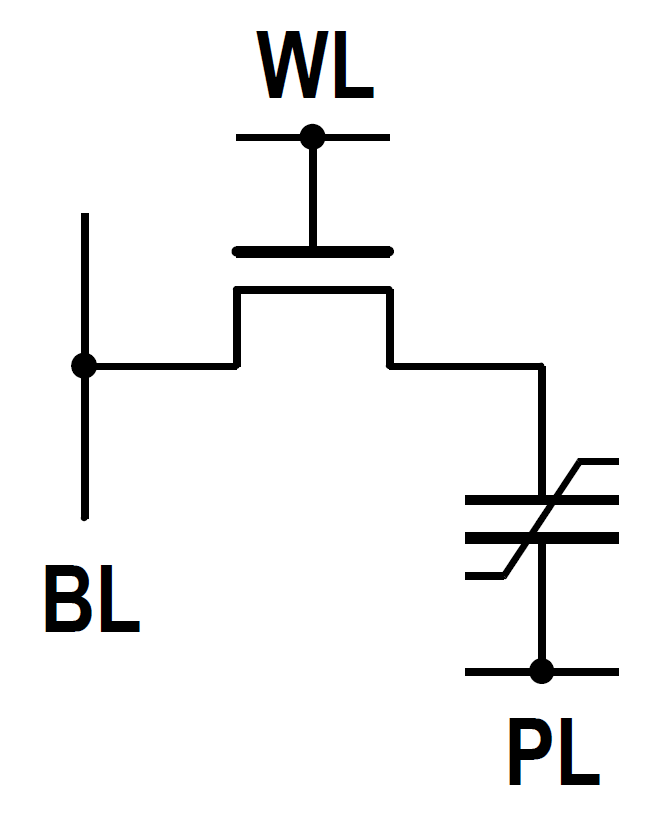
\includegraphics[width=\textwidth]{FRAM-fig1.png}
    \caption{Схематический вид}
    \label{pic:cell_sc}
  \end{subfigure}
  %
  \begin{subfigure}[b]{0.8\textwidth}
    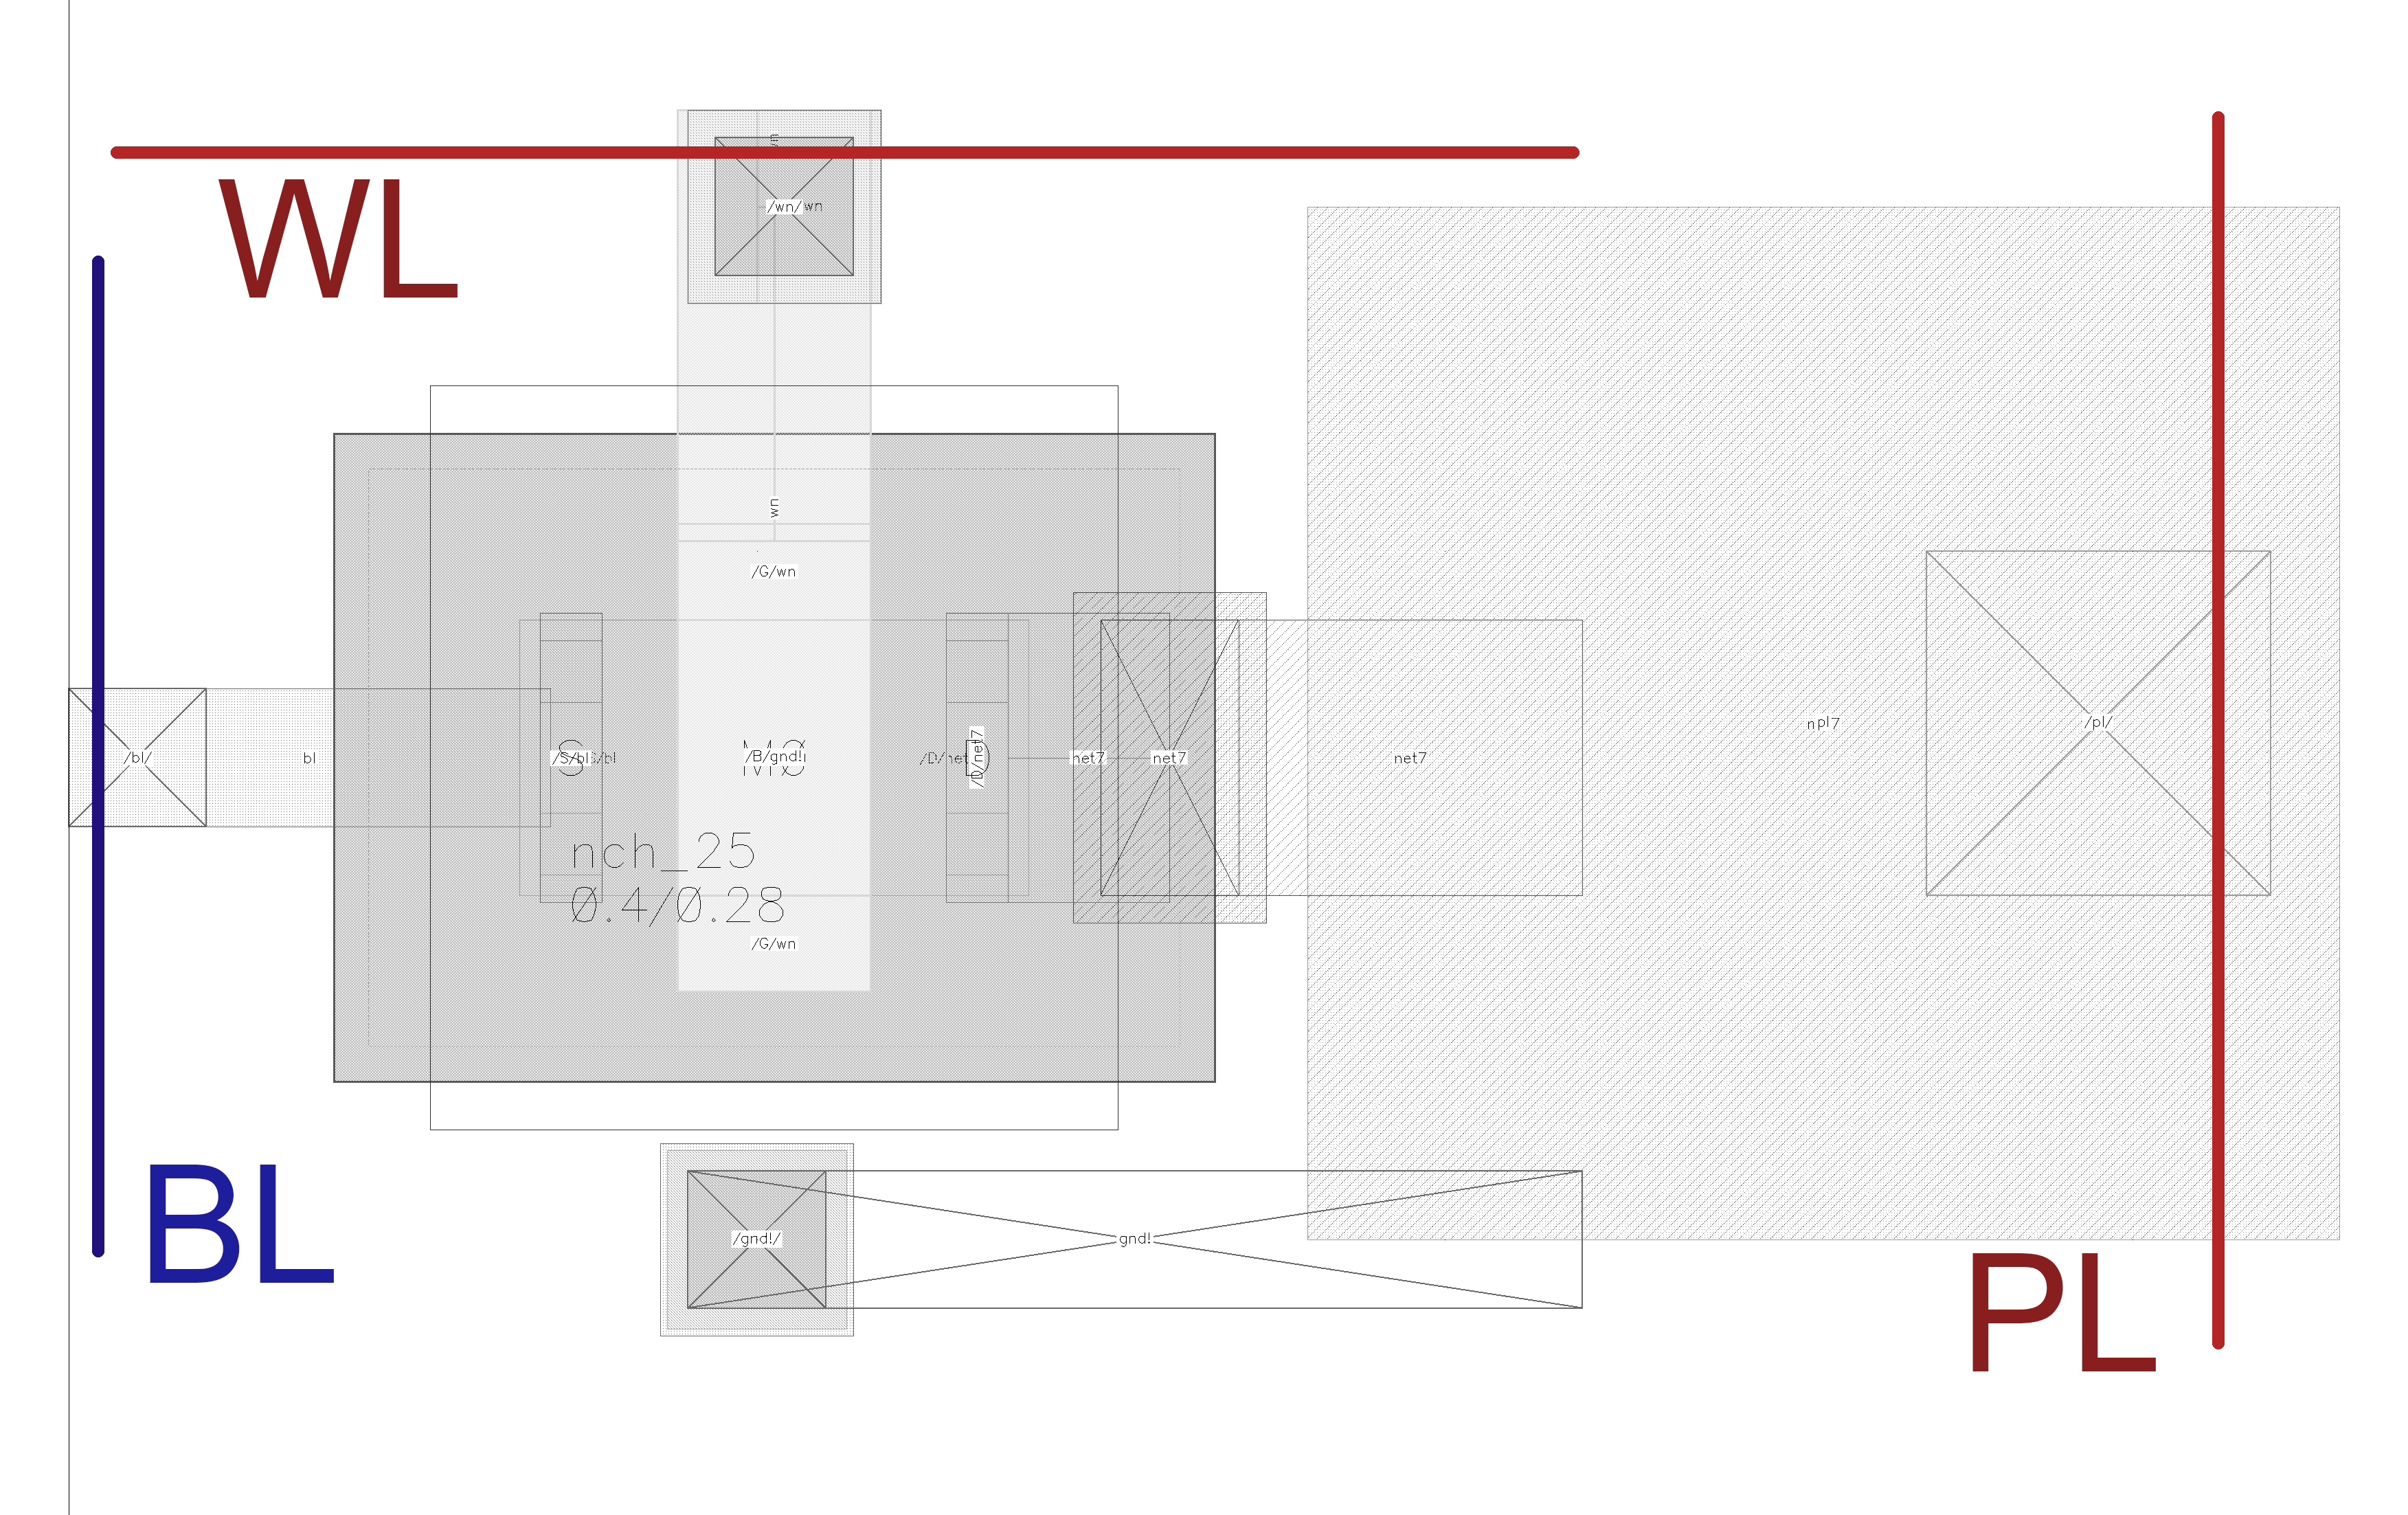
\includegraphics[width=\textwidth]{cell.png}
    \caption{Топология на кристалле}
    \label{pic:cell_la}
  \end{subfigure}
  \caption{Ячейка FRAM памяти реализованная в тестовом чипе}
\end{figure}




\subsubsection{Усилитель чтения} %РИСУУУУНКИ!!
\label{subsec:amp}
Цифровой дифференциальный компаратор, показанный на рисунке \ref{amp:2} , используется в DRAM как
также как SRAM. Исток верхнего p канального транзистора подключчется  к источнику питания, и его сток подключчается к левой и правой ветви. Каждая ветвь включает в себя два последовательно соединенных p-канальных транзистора, за которыми следуют два параллельно соединенных n-канальных транзистора. Однако эта схема обычно находит применение на линии данных, внешнем по отношению к самому массиву памяти, усиливая сигнал данных, полученный из массива памяти, и передавая его.
на выходной буфер. Поскольку в этой схеме отсутствует какая-либо возможность обратной записи на входные узлы, и поскольку она несколько сложнее, чем традиционная защелка.
Усилитель, показанный на рисунке \ref{amp:1} , обычно не находит применения в самом массиве памяти. Однако этот компаратор имеет явные преимущества по сравнению с усилителем на защелке. Основным преимуществом, которым он обладает, является его скорость при усилении
небольшого дифференциального входного сигнала. Поскольку выходные узлы или узлы фиксации компаратора, узлы NT и NB, как правило, слегка загружены емкостно, они очень
быстро доводится до  уровня выходной логики. Отделяя не сильно
загруженный выход с сильно загруженного входа, компаратор способен быстро усиливать
малый дифференциальный входной сигнал и установить большой дифференциальный выходной сигнал.
Есть несколько характеристик сегнетоэлектрической памяти, которые делают приложение
из компаратора выгодным.


\begin{figure}
  \begin{subfigure}[b]{0.48\textwidth}
    \includegraphics[width=\textwidth]{comparator.png}
    \caption{Усилитель неразрушающего чтения (используется в нашем устройстве памяти)}
    \label{amp:1}
  \end{subfigure}
  %
  \begin{subfigure}[b]{0.5\textwidth}
    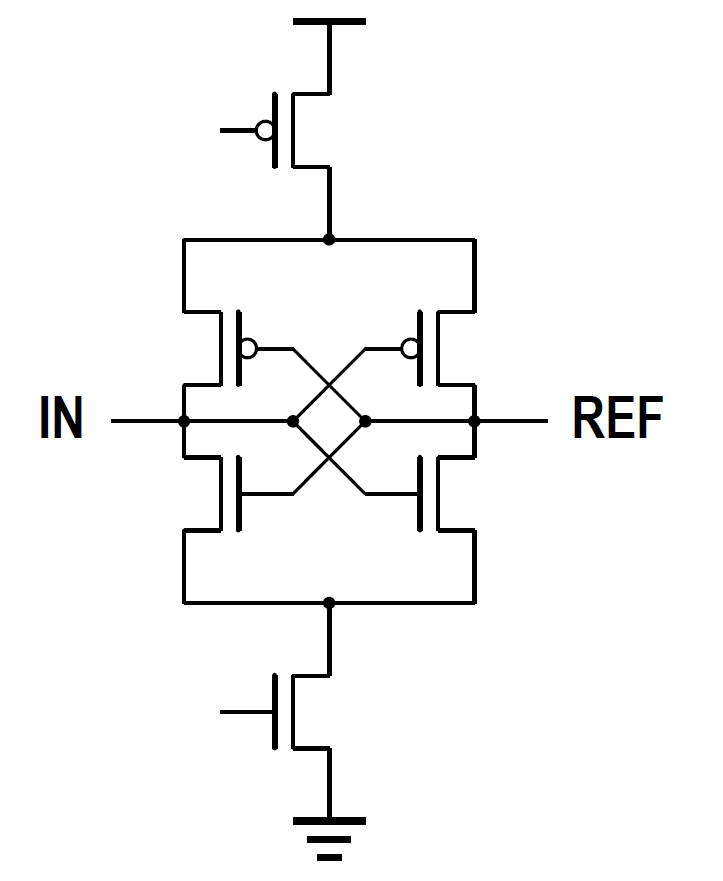
\includegraphics[width=\textwidth]{SemAmp.png}
    \caption{Усилитель на защелке (используется в DRAM и SRAM).}
    \label{amp:2}
  \end{subfigure}
  \caption{Схемы усилителей чтения}
\end{figure}

\subsubsection{Недостатки обычного усилителя чтения}
Как правило, в DRAM битлайны предварительно заряжаются до уровня  $\frac{V_{dd}}{2} $ до чтения. Этот уровень обычно достаточно высок, чтобы n-канальные устройства с перекрестными связями в усилителе считывания могли усиливать разностный сигнал. Так как мобильность n-канальных транзисторов обычно в два-три раза больше, чем у p-канальных транзисторов,
большая часть усиления происходит от пары n-каналов, а не от p-канала,
аналогично для одновременной активации обеих пар. Однако в случае FeRAM разрядные линии предварительно заряжены на землю  для более высокого коэрцитивного напряжения. Следовательно, измерение и усиление с помощью N-канала невозможно, поскольку результирующие напряжения разрядной линии равны или ниже пороговых напряжений n-канального МОПа. Если бы использовался традиционный усилитель с защелкой, считывание и усиление выполнялись бы исключительно с помощью пары кросс-связанных p-каналов, тем самым снижалась бы чувствительность усилителя и скорость усиления.



\subsubsection{Генератор референсных сигналов}

Генератор опорного напряжения на кристалле способен генерировать ряд возрастающих напряжений от VREFP до VREFM и в основном используется в комбинации со схемой распределения заряда.  Его выход VREF подключен к входу опорного напряжения всех усилителей чтения.  Несмотря на большую выходную ёмкость, генератор опорного напряжения по-прежнему способен изменять выходное напряжение в течение примерно 2 нс.

В качестве внутреннего генератора сигнала была выбрана простейшая 8-ми битная R2R цепочка состоящая  из резисторов в слое поликремния. Чтобы понять что 8 битов достаточно для того чтобы хорошо покрыть точность измерения. 6 битов дают 64 разных значения напряжения. То есть шаг при этом будет вычиляться как $$ \frac{V_{dd}}{N}=\frac{2.5}{128}\approx 20 mV $$
Что примерно равно максимально возможно различимому сигналу для усилителя (см. \ref{sec:noise})

Схема такого цифро-аналогового преобразователя представлена на рисунке \ref{pic:r2r}.

\begin{figure}[H]
\centering
  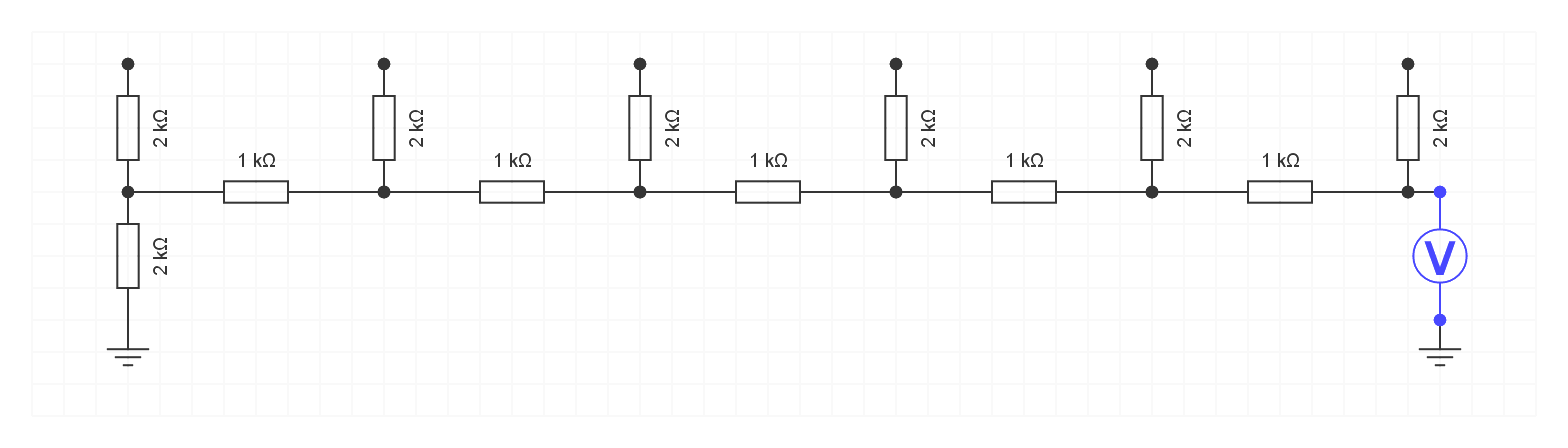
\includegraphics[width=\linewidth]{r2r.png}
  \caption{Cхема устройства 6ти битного  R2R преобразователя}
  \label{pic:r2r}
\end{figure}

\subsection{Топология чипа}
\label{sec:layout}
\subsubsection{Выбор техпроцесса}
\label{subsec:DK}
Первоначально предполагалось реализовать layout чипа на техпроцессе <<Микрон 90нм>>, однако на данный момент от этой идеи пришлось отказаться в виду сложности работы моделей этого техпроцесса со смешанной аналого-цифровой симуляцией, что делает сложным проектирование прототипа памяти. Поэтому решено было изготовить схему проекта на техпроцессе <<TSMC 65 nm>>. Данный техпроцесс содержит в себе все необходимые элементы для создания памяти, в том числе спайс модели для их симуляции, и возможность работать с layout моделями. Так же одна из причин выбора данного техпроцесса возможность верификации его (подробнее ~\ref{subsec:veryf} ) путем DRC и LVS верификаций.

\subsection{Верификация Дизайна}
\label{subsec:veryf}


\subsubsection{LVS}

LVS (layout versus schematic) используется для проверки того, что топология проекта соответствует изначально  схеме во всех возможных аспектах (соединения сигналов, размеры транзисторов, емкости, имена сигналов и т. Д.) И что во время создания топологии не было ошибок. Если есть
ошибки в оформлении, которые ухудшают функциональность чипа, которые не учиены в проекте, то предпринимаются меры по устранению ошибок layout.
На схеме они не могут быть найдены с помощью схемотехнического моделирования. LVS выявляет любые различия между топологией и чипос и тем самым позволяет разработчку
исправить либо топлогию, либо схему - в зависимости от того, что не так.
Полная проверка LVS была выполнена с использованием  нетлистов для топлогии и
изначальной схемой памяти. Этот процесс также очень вычислительно ёмкий, так как этап извлечения нетлиста для топологии занимает время. После того как созданы оба нетлиста, они
сравниваются друг с другом, и любые различия помечаются как ошибки или предупреждения. После устранения обнаруженных расхождений весь процесс должен повторяться до полной верификации чипа.


\subsubsection{Экстракция паразитных параметров}
\label{subsec:parasitic}
Как только LVS верификация  проведена успешно, проводитсья экстракция паразитных параметров. Переход от изначальной  схематики  к топологии сопровождается приобритением любой схемой паразитных параметров: проводники превращаются в резисторы и конденсаторы. Иногда этот эффект может быть очень значительным для дизайна, или же наоборот использоваться в целях устройства. Так например битовая линия которая для успешной работы прибора должна иметь четко определенные параметры ёмкости. Для того чтобы заранее предусмотреть влияние паразитных параметров существует так называемая экстракция паразитных параметров. На уровне техпроцесса задаются удеальные паразитные параметры, после чего используется специальный экстрактор паразитных параметров, который эксплуатируя  удельные параметры получает новую схему содержащую помимо заложенных дизайнером схему так же набор параметров.  В нашем проекте в качестве экстрактора был использован модуль PEX Calibre, который встраивается в среду Cadence Virtuoso.



\section{Анализ оптимизации чипа памяти}
\label{sec:analisis}
\subsection{Цели анализа: шум усилителя как основной ограничивающий фактор}
\label{sec:noise}
Как и везде шум является основным ограничевающим фактором. Как и в описанном в главе ~\ref{sec:dram}
Таким образом шум усилителя ограничевает как возиожность работы устройства как памяти, так и работу его как устройство измерения заряда. Для корректной работы компаратора разница сравниваемых напряжений должна быть больше интегрального шума по частотам работы компаратора. 
$$ \Delta V = |V_{ref} - V_{in}| < V_{noise}  $$
, где $V_{noise}$ (эффективное влияние шума)вычесляется как интеграл по спектральной плотности шума, в пределе эффективных частот его работы.
$$ V_{noise,total}^2 = \int_{\omega_1}^{\omega_2} V_{noise}^2df   $$
Где $V_{N2}$, есть спектральная характеристика шума усилителя.

Таким образом можно считать, что шум является ограничивающим фактором, причем сразу в трех направлениях: Скорость работы, плотность ячеек и их размер. Поэтому именно его оценка является определяющей для проектирования аналоговой части чипа. 



\begin{figure}[H]
  \begin{center}
    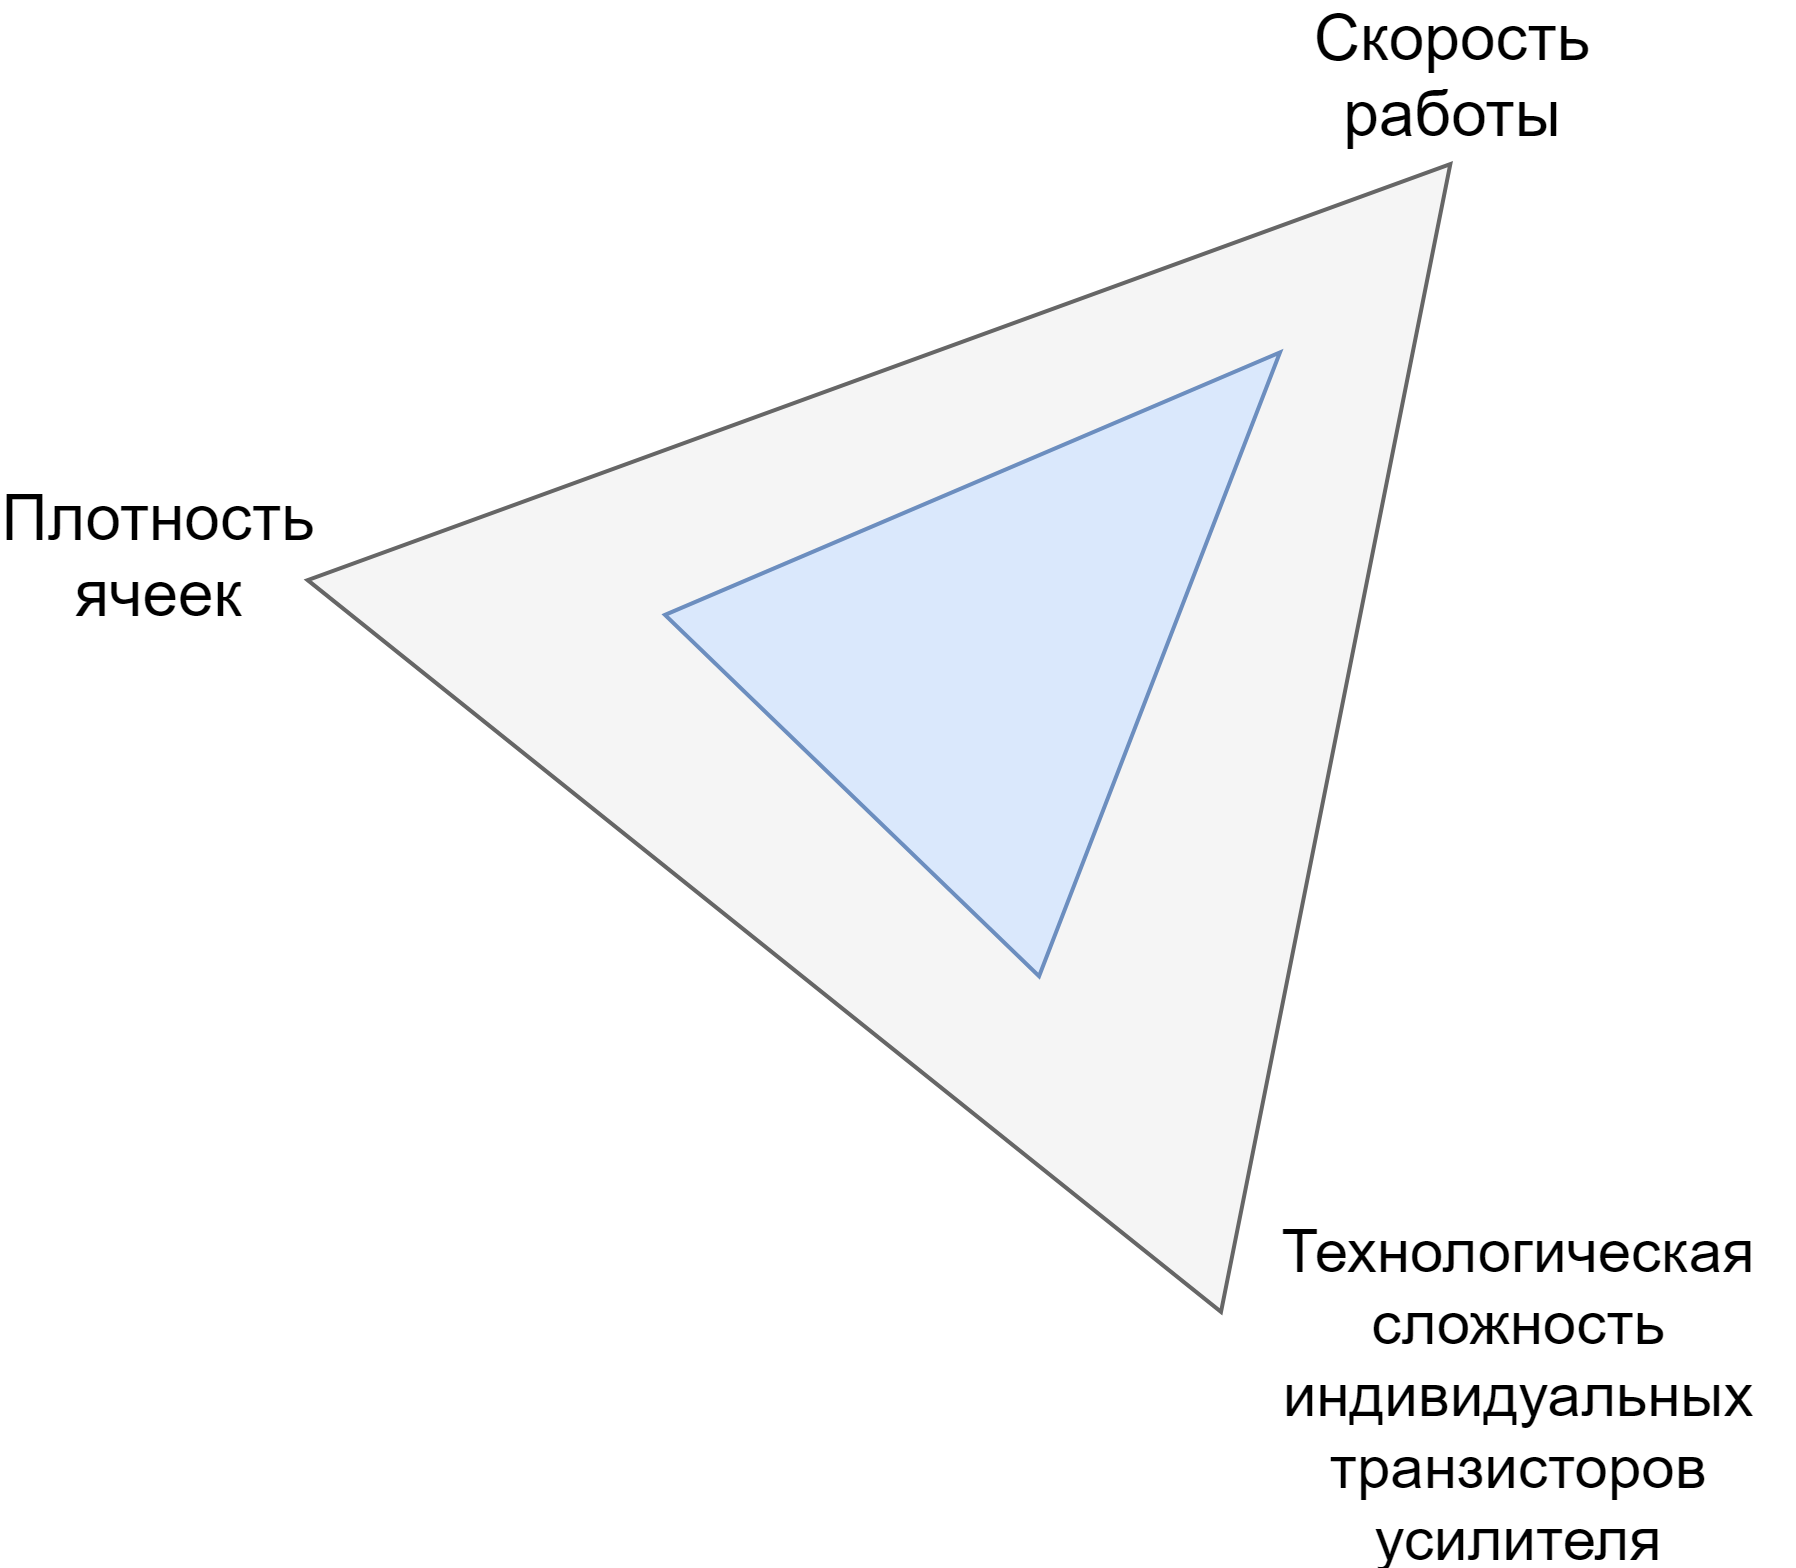
\includegraphics[width=0.6\linewidth]{FRAM-6.png}
  \end{center}
  \caption{Трейдофф дизайна вызванный шумами }
  \label{FRAM_fig6}
\end{figure}

Таким образом на этапе проектирования схемотехники критично 
 
\subsubsection{Проблема поиска шума усилителя использованного в тестовом чипе и симуляция с использованием метода Монте Карло}

Как описано в предыдущем параграфе поиск шума при разработке чипа является критичным аспектом оценки возможности его реализации. Усилитель использованный в разработке тестового чипа описанный в главе \ref{subsec:amp} , не является линейным усилителем, вместо этого он представляет собой бинарный компаратор с защелкой. То есть обратная связь мешает нам получить шумовую характеристику на выходе, и каким то образом ее нужно разорвать, это один из способов получения шумовых характеристик для нелинейных усилителей. К сожалению оказалось что невозможно разорвать обратную связь данного усилителя не повлияв на его передаточную функцию. Исходя из этой особенности пришлось пойти другим путем, используя временную симуляцию с методом Монте Карло \cite{carlo}. При этом суть метода состоит в интеграции стохастического процесса во временной анализ и повторение данной симуляции многократно. Подробнее о способе анализа котой мы использовали для оценки производительности усилителя в части \ref{subsec:amp_noise_test}. При этом результат предоствляется в виде так называемого "Шму графика", представляющего результат бинарного теста по двум параметрам.



\subsection{План Анализа}



\subsection{Результаты Анализа}

\subsubsection{Результат анализа шумовых характеристик усилителя}
\label{subsec:amp_noise_test}

Таким образом для достоверного анализа возможности работы усилителя в заданных условиях была проведена временная симуляция с моделированием шумов по методу Монте Карло \cite{carlo}. То есть шумы добавлялись непосредственно во временной анализ, после чего симуляция  проводилось порядка 200-300 раз. Если все 200 считываний расхождений в работе усилителя обнаружно не было, данный тест признавался пройденным (пример безошибочного считывания в условиях работы близких к критическому на рисунке \ref{pic:ok}). Если же при этом хоть один раз считывание происходило ошибочно (пример ошибочного считыванния на рисунке \ref{pic:fail} то данный набор частот клока и считываемого напряжения признавался за гранью предельного для усилителя. Если же из 200 прогонов все оказывались достоверными, то можно считать что данная частота и разность напряжений все еще способны считываться усилителем. Для данного измерения было взято сравнение с референсным напряжением 30мВ, при емкостях нагрузки в $50 fF$. Такая емкость была выбрана чтобы исключить влияние невозможности считывания из за слишком большой ёмкостной нагрузки, ибо при частоте работы в 1ГГц ёмкость в 500фФ попросту не успевает заряжаться, по нашим рассчетам (подробнее в главе про основы дизайна FRAM) емкости в $~5\cdot10^{-14}=50fF  $  должно , при текущей технологии  хватить на размещение более 250 ячеек, что более чем достаточно для высоты одного массива. Более подробные данные о емкостях битовой линии и остаточном заряде ячейки в пункте \ref{subsec:c_bl} . Окончательные данные о проведенном тесте предствлены на рисунке \ref{pic:shmoo}




\begin{figure}
  \begin{center}
    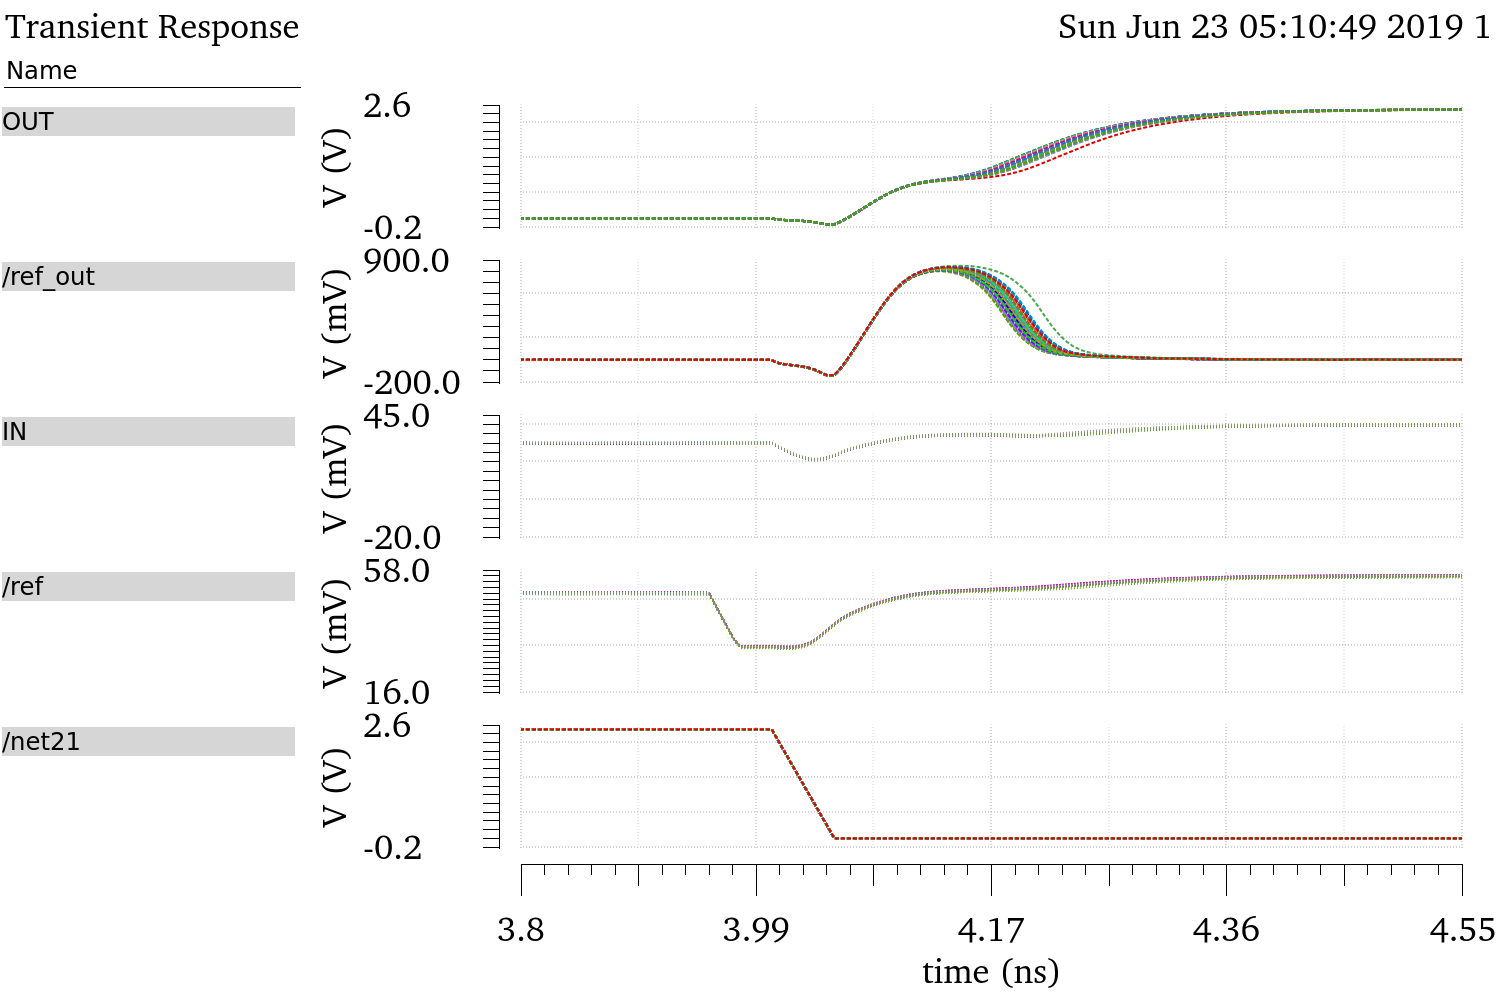
\includegraphics[width=0.8\linewidth]{ok.png}
  \end{center}
  \caption{Пример успешной работы усилителя несмотря на близкие к предельным значения сравниваемого напряжения $V_{in}=50mV $ $ V_{ref}=30mV $ $C_{in}=50fF $}
  \label{pic:ok}
\end{figure}

\begin{figure}
  \begin{center}
    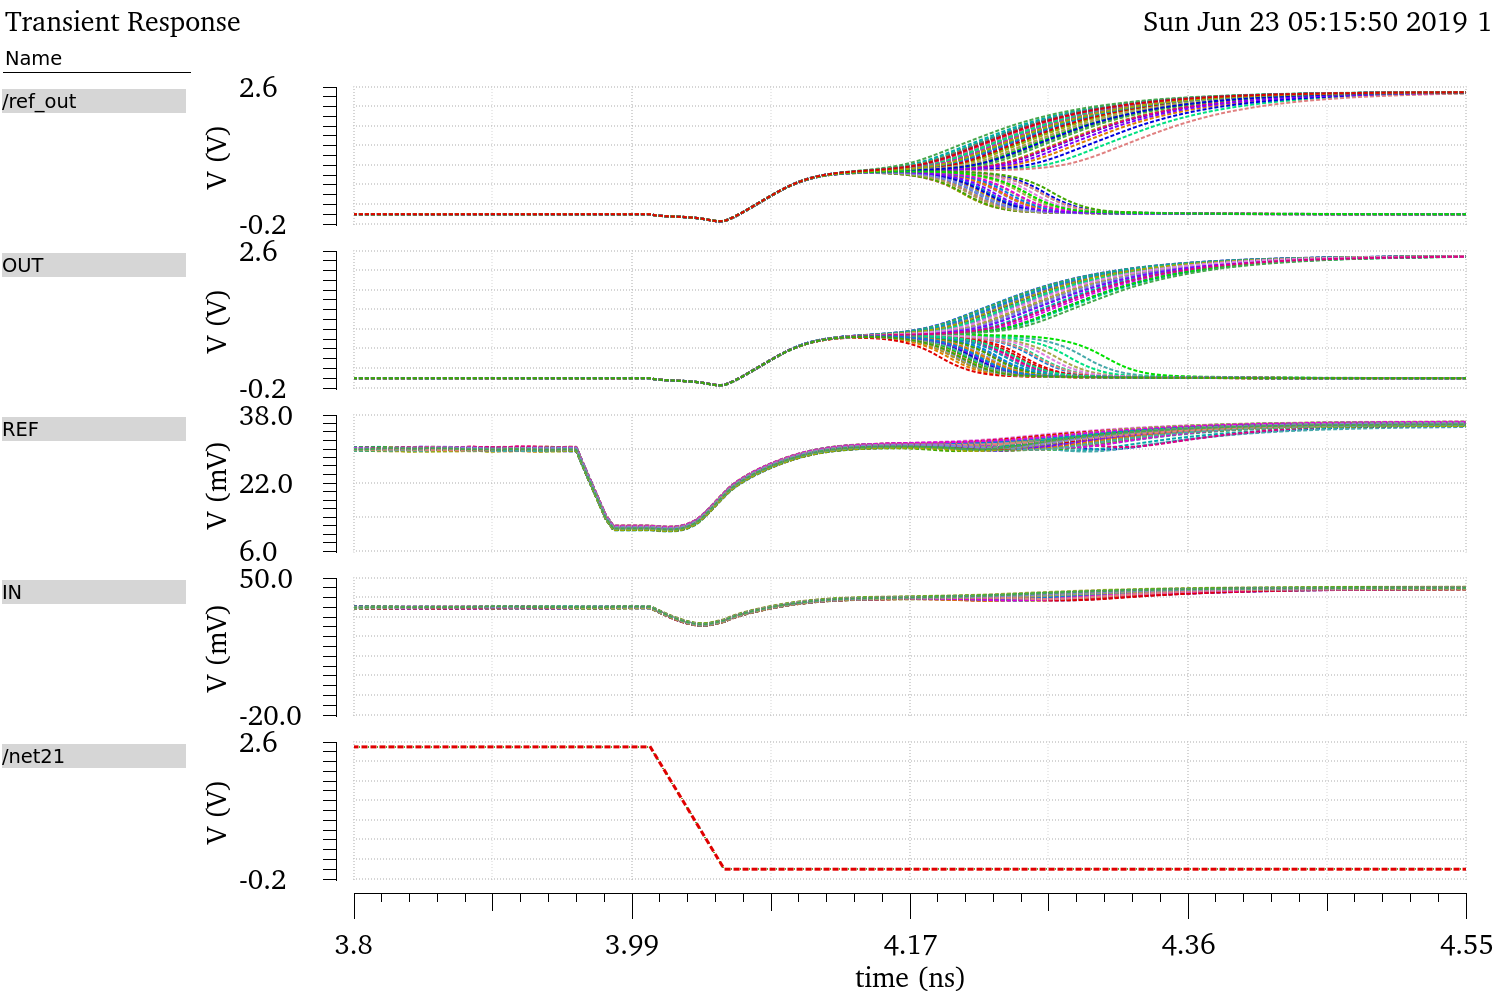
\includegraphics[width=0.8\linewidth]{fail.png}
  \end{center}
  \caption{Пример расщипления результатов теста при $ \Delta V <15mV $, как видно шумы приводят к тому что в ряде случаев усилитель более не может корректно сравнить два наапряжения: $V_{in}=40mV $ $ V_{ref}=30mV $ $C_{in}=50fF $}
  \label{pic:fail}
\end{figure}





   \begin{figure}[H]
   \centering
  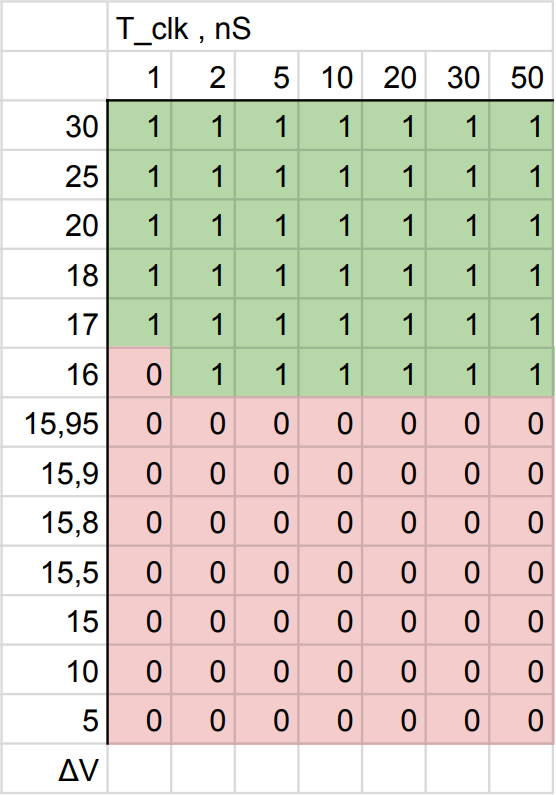
\includegraphics[width=0.5\textwidth]{shmoo.png}
  \caption{Анализ успеха чтения усилителя при разной разности напряжений $\Delta V , mV $ и разных временах клока контроллера $T_{clk}, nS$ \colorbox{LimeGreen}{зеленым} успешное чтение при всех 200 симуляциях, \colorbox{BrickRed}{красным}, напряжения которые усилитель на данной частоте более не может сравнить}
  \label{pic:shmoo}
  \end{figure}


Как станоситься видно из рисунка \ref{pic:shmoo} , сравниваемое напряжение в большей  степени влияет на успех тестов нежели частота. Ибо как видно даже порядок частот работы более чем в 10 раз не так сильно сказывается на работе как повышение сравниваемого напряжения на целый $1 mV $. На тактовых частотах ниже 5нс становиться критичным баланс между входной емкостью, ибо напряжение попросту может не успеть вырасти до нужного , даже при ёмкости в  $0,5 pF $. 

\subsubsection{Анализ отношения ёмкости битовых линий, размера ячеек и достоверности чтения}
\label{subsec:c_bl}
В главе \ref{sec:fram} было описано, что при создании FRAM  приходится брать в учет баланс между плотностью, скоростью, надежностью (фактически возможностью работы). В ходе подготовки итогового дизайна нужно было найти необходимый компромисс между размером ячеек, их количества на одной линии. Для этого был проведен следующий параметрический анализ: для четырех различных емкостей битлайна (50,100,200,500 фФ), для различных значений размеров ячейки замерялся заряд сброшенный при чтении двух состояний. При чтении единицы $V_1$ (1), и при чтении нуля $V_2$ (0). Далее это повторялось для различных значений размеров ячейки (S), в пределах длинны ячейки от 500 до 100 нм, данные о которых представлены как в виде Талицы \ref{tab:c_bl} так и в виде графика (рис. \ref{pic:c_bl}).

% Please add the following required packages to your document preamble:
% \usepackage{multirow}
\begin{table}[h]
\centering
\begin{tabular}{|l|l|l|l|l|l|l|l|l|l|l|}
\hline
\multicolumn{3}{|l|}{}                                                        & \multicolumn{8}{l|}{$V_{BL},mV$}                                                                                 \\ \hline
\multirow{2}{*}{p0,$\frac{uC}{cm^2} $} & \multirow{2}{*}{S,$M^2$} & $C_{BL}$: & \multicolumn{2}{l|}{50fF} & \multicolumn{2}{l|}{100fF} & \multicolumn{2}{l|}{200fF} & \multicolumn{2}{l|}{500fF} \\ \cline{3-11} 
                                       &                          & L,M       & V1(1)       & V2(0)       & V1(1)        & V2(0)       & V1(1)        & V2(0)       & V1(1)        & V2(0)       \\ \hline
25                                     & 2,50E-13                 & 5,00E-07  & 305         & 77          & 177          & 33          & 1143         & 96          & 521          & 17          \\ \hline
25                                     & 1,50E-13                 & 3,87E-07  & 210         & 50          & 1318         & 130         & 762          & 38          & 318          & 5           \\ \hline
25                                     & 1,00E-13                 & 3,16E-07  & 157         & 40          & 978          & 70          & 518          & 22          & 214          & 5,9         \\ \hline
25                                     & 5,00E-14                 & 2,24E-07  & 942         & 78          & 513          & 30          & 270          & 12          & 110          & 4,2         \\ \hline
\end{tabular}
\caption{Зависимость разности заряда между нулем и единицей при разных размерах ячейки и разных емкостях битовой линии}
\label{tab:c_bl}
\end{table}

\begin{figure}
  \begin{center}
   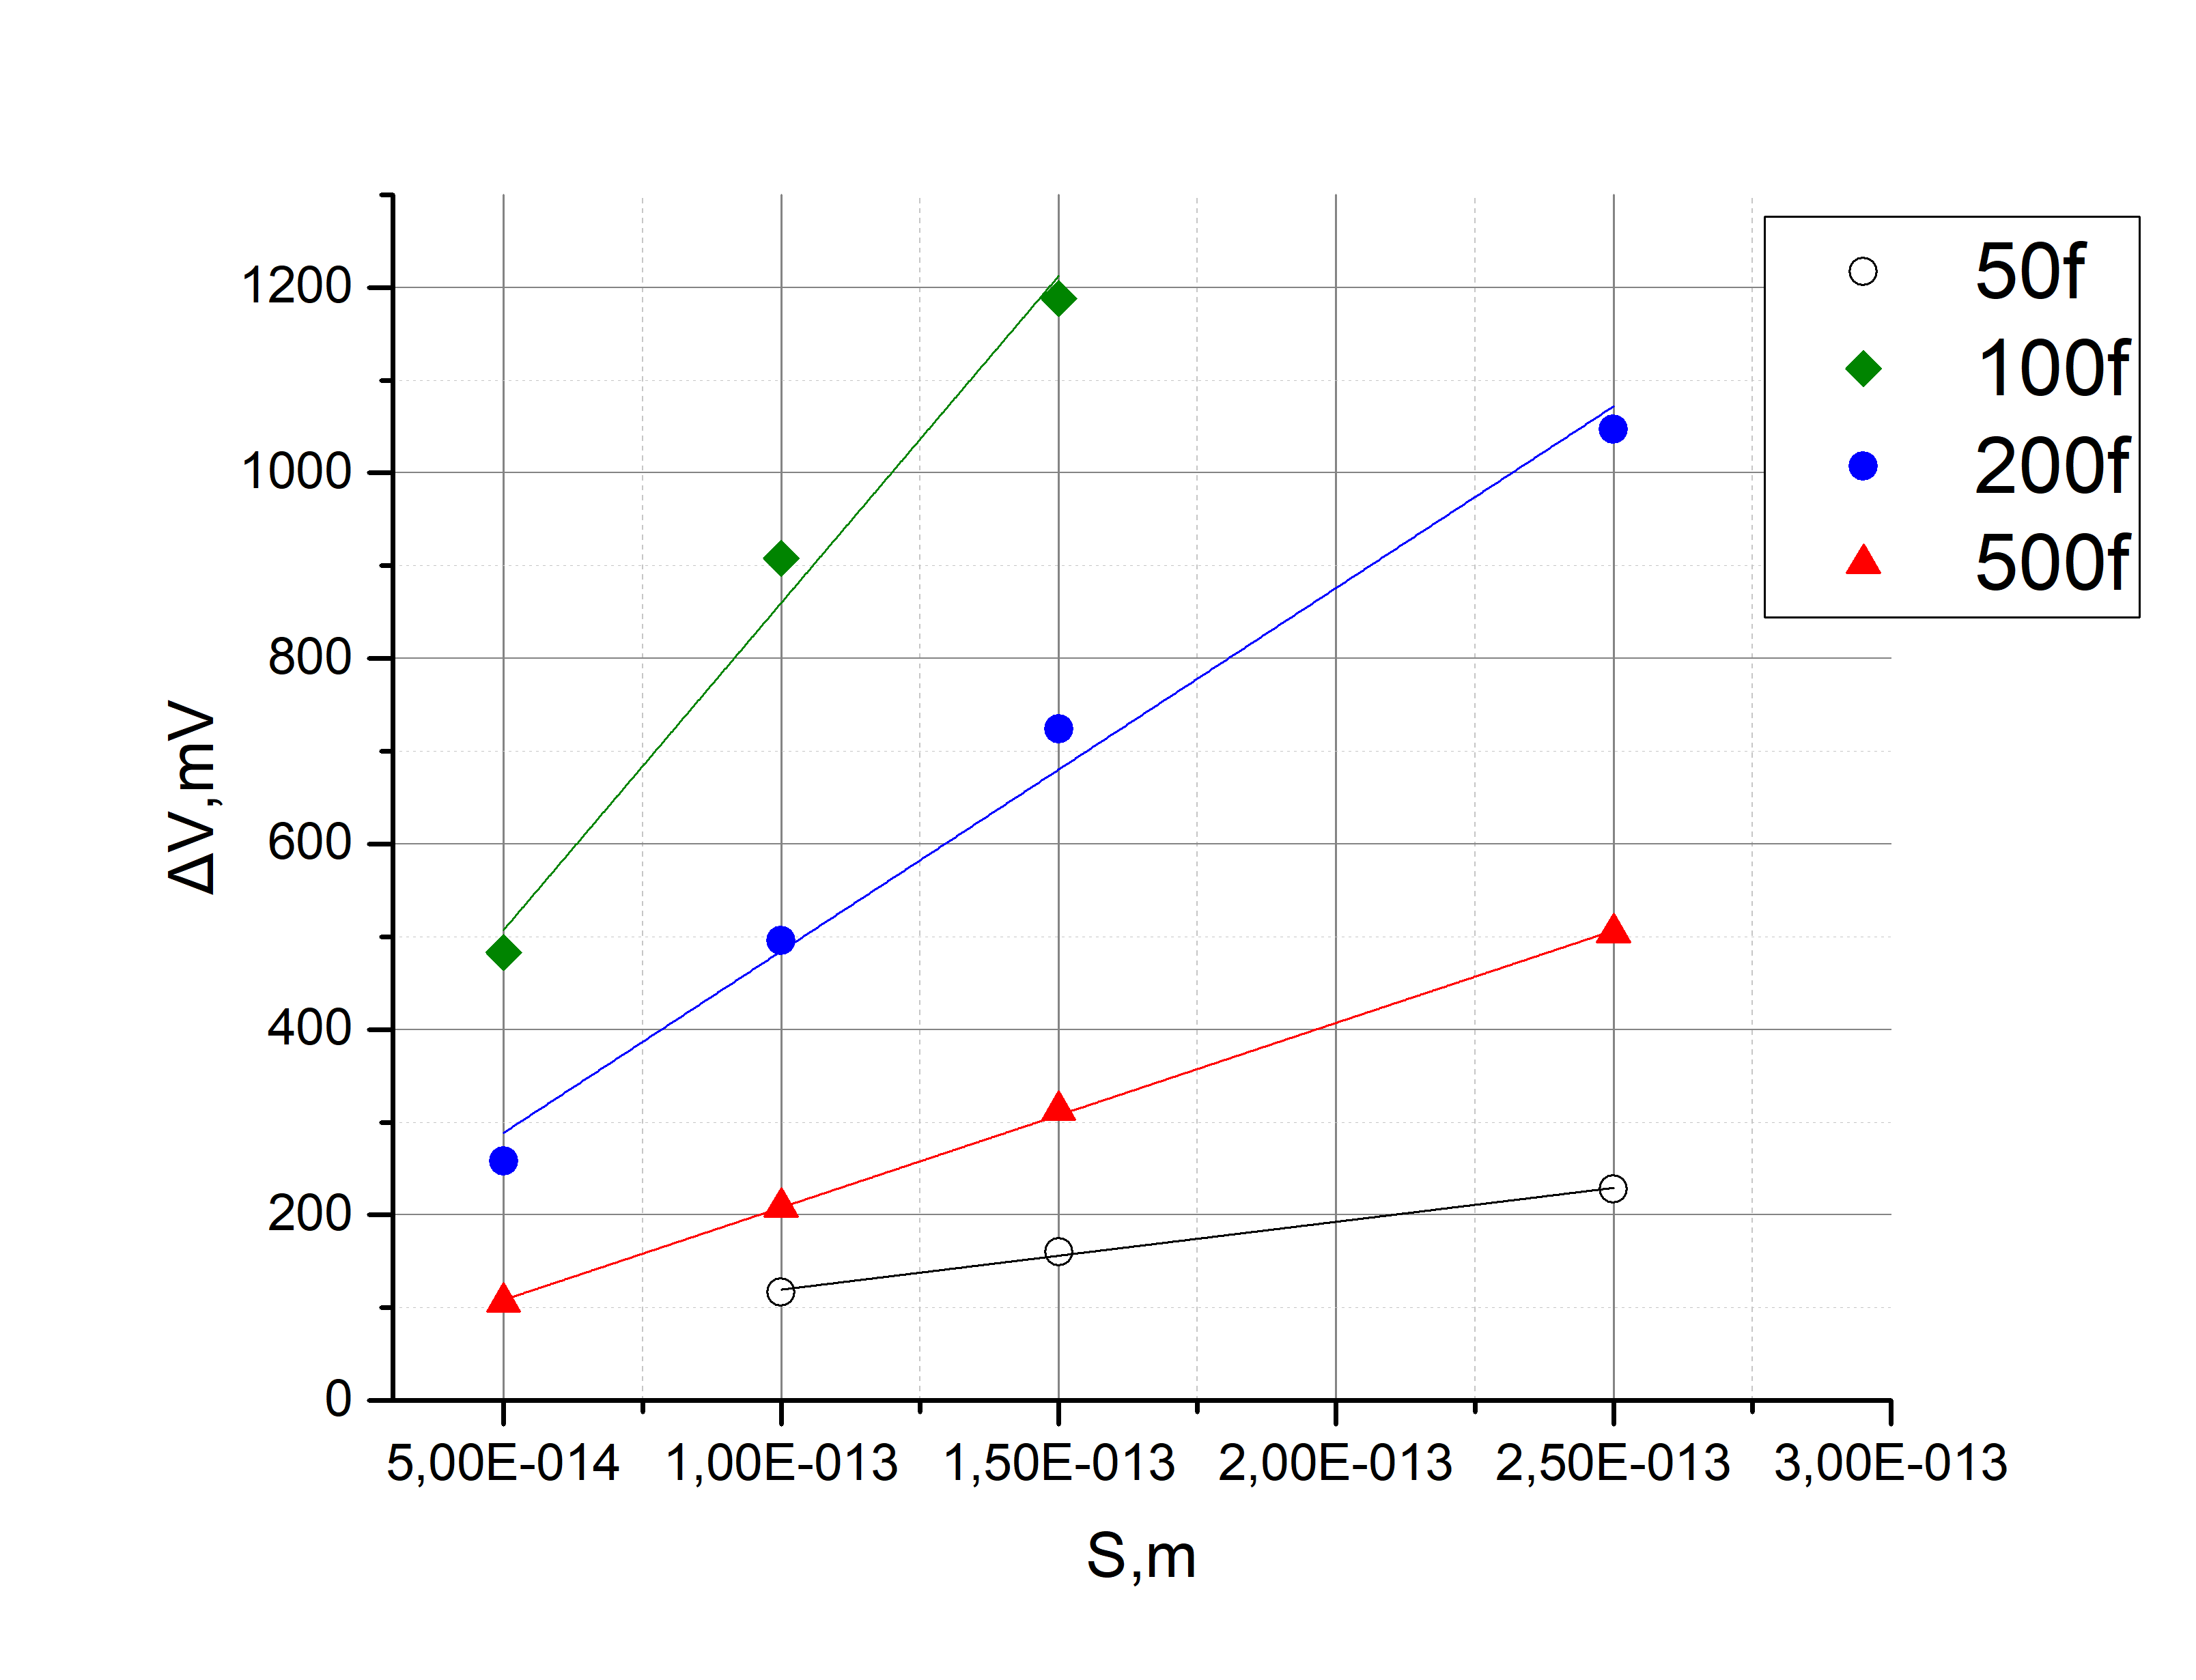
\includegraphics[width=\linewidth]{c_bl.png}
  \end{center}
  \caption{представление таблицы \ref{tab:c_bl} в виде графика }
  \label{pic:c_bl}
\end{figure}





Как видно избыточно малая или большая ёмкость приводит к уменьшению зазора напряжения между 0 и 1. При большой ёмкости это следствие закона сохранения заряда: заряд ячейки превращается в малое напряжение в виду большой емкости битовой линии. Численно данная закономерность описана в главе \ref{sec:dram}. Так же при избыточно малой емкости, значительной становиться нижняя граница напряжение на которую начинают влиять малейшие шумы и утечки (учитывались в процессе анализа). Таким образом данный анализ помогает нам выбрать идеальную емкость битлайна. Причем большая ёмкостная нагрузка будет обеспечивать прибору большую защещенность от помех (особенно при чтении нуля), но в то же время будет особенно сильно влиять на максимальную частоту работы, ибо при емкости в $500fF$  на частоте работы в 1 ГГц входной терминал усилителя чтения попросту не успеет зарядиться даже до напряжения 200mV, таким образом нам приходиться еще брать в учет пробемы ограничения частоты при использовании большой ёмкости. Так же при создании прибора с малой емкостью битовой линии придется еще сильнее учитывать ранее не актуальную ёмкость ячейки памяти как конденсатора, которая при увеличении частоты может так же вностить вклад в напряжение битлайна (напряжение попросту не будет успевать стекать обратно в ячейку ).


\section{Итоги работы}

Я надеюсь эта работа найдет реализацию в развитии технологии полупроводниковой памяти, для чего в ней были получены следующие результаты:

\begin{enumerate}


	\item Произведен обзор основных проблем  создания динамической памяти на сегнетоэлектрических технологиях и их решения (см. \ref{sec:fram}).
	\item Освоен способ относительно достоверной симуляции сегнетоэлектрического конденсатора при аналоговой спайс симуляции.
	\item Произведена оценка отношения плотности памяти и объема ее ядер для тестового образца (см. \ref{subsec:c_bl}).
	\item Произведена оценка возможности стабильной работы усилителя, а как следственно частотный и габаритный предел создания FRAM на данной технологии.
	\item Создана топология для запуска тестового чипа в производство.
\end{enumerate}

Основным лимитирующим фактором для создания данного чипа сейчас является только не интегрированность сегнетоэлектрических конденсаторов в существующий техпроцесс. Однако общая популярность чем то схожей в конструкции DRAM памяти может дать необходимую базу для стремительного развития данной технологии, особенно в местах где необходима большая частота записи данных, и больщой ресурс работы энергонезависимой памяти.








\newpage
\appendix
\section{Дополнение}
\subsection{Код для симуляции поведения сегнетоэлектрика}

\subsubsection{Код в Python}
\begin{lstlisting}[language=Python]
# -*- coding: utf-8 -*-
"""
Created on Mon Apr 16 18:34:51 2018

@author: Mikhail Solovyanov
"""

import matplotlib.pyplot as plt
import numpy as np
from scipy.optimize import fsolve
from scipy.integrate import odeint


num=1000


E_c = 1/8

P_0 = 1

R = 0.001

alpha = (np.sqrt(27/4)*(E_c))/P_0
beta = (P_0**2)*alpha

t= np.linspace(0, 10, num)
#t = np.linspace(0, itimes[-1], num)
p=np.zeros(len(t))
def u(t):
    return np.sin(t)*1
    #return np.interp(t, itimes, ivolts)
    
def u_i(t,i):
    return np.sin(t[i])*1

U=u(t)

#alpha = 0.5
#beta = 0.5

def gibbs(p,t):
    return (-beta*p**3 + alpha*p + u(t)) / R

p[0]=0

p = odeint(gibbs,0,t)
p = p[:, 0];
j=np.zeros(len(t))
j = np.concatenate(([0], np.diff(p)))

#for i in range(len(t)):
#   j[i]= (p[i]-(p[i]**3)+u_i(t,i))
uvec = list(map(u, t))

plt.clf()
#print(p)
plt.plot(t, uvec, label = 'p')
plt.plot(t, j, label = 'j')
plt.plot(t, U, label = 'U')
#plt.plot(uvec, p, label = 'j')
plt.grid(True)
plt.legend()
plt.savefig("fsolve.png")
plt.show()
\end{lstlisting}
\newpage
\subsubsection{Код симуляции поведения конденсатора  на языке veylogA}
\begin{lstlisting}[language=Verilog] 
`include "disciplines.vams"

module conder (a, b) ;
	inout a, b ;
	electrical a, b ; // access functions are V() and I()

	parameter real Ec = 2;
	parameter real dT = 1e-9;
	 
	parameter real p0 = 1e-12;
	
	localparam real alpha = 3*sqrt(3)*Ec/(8*p0*p0*p0);
	localparam real beta = -3*sqrt(3)*Ec/(4*p0);
	

	real p;
	real de;
	real Rdamp;

	analog begin
		//@(initial_step("tran")) p = p0;
		de = V(a, b) - 2*beta*p - 4*alpha*p**3;
		Rdamp = (+beta+(24*alpha*p0*p0))*dT;
		p = idt(de/Rdamp, p0);
		I(a, b) <+ ddt(p);
//		$display(p);
//		$display("%e %e", p0, p);

	end
	
endmodule

\end{lstlisting}

\subsection{Топология столбца памяти}
Данная топлогия для того чтобы уместиться здесь содержит 6 ячеек, однако способна маштабироваться наверх.
\begin{figure}[H]
  \begin{center}
    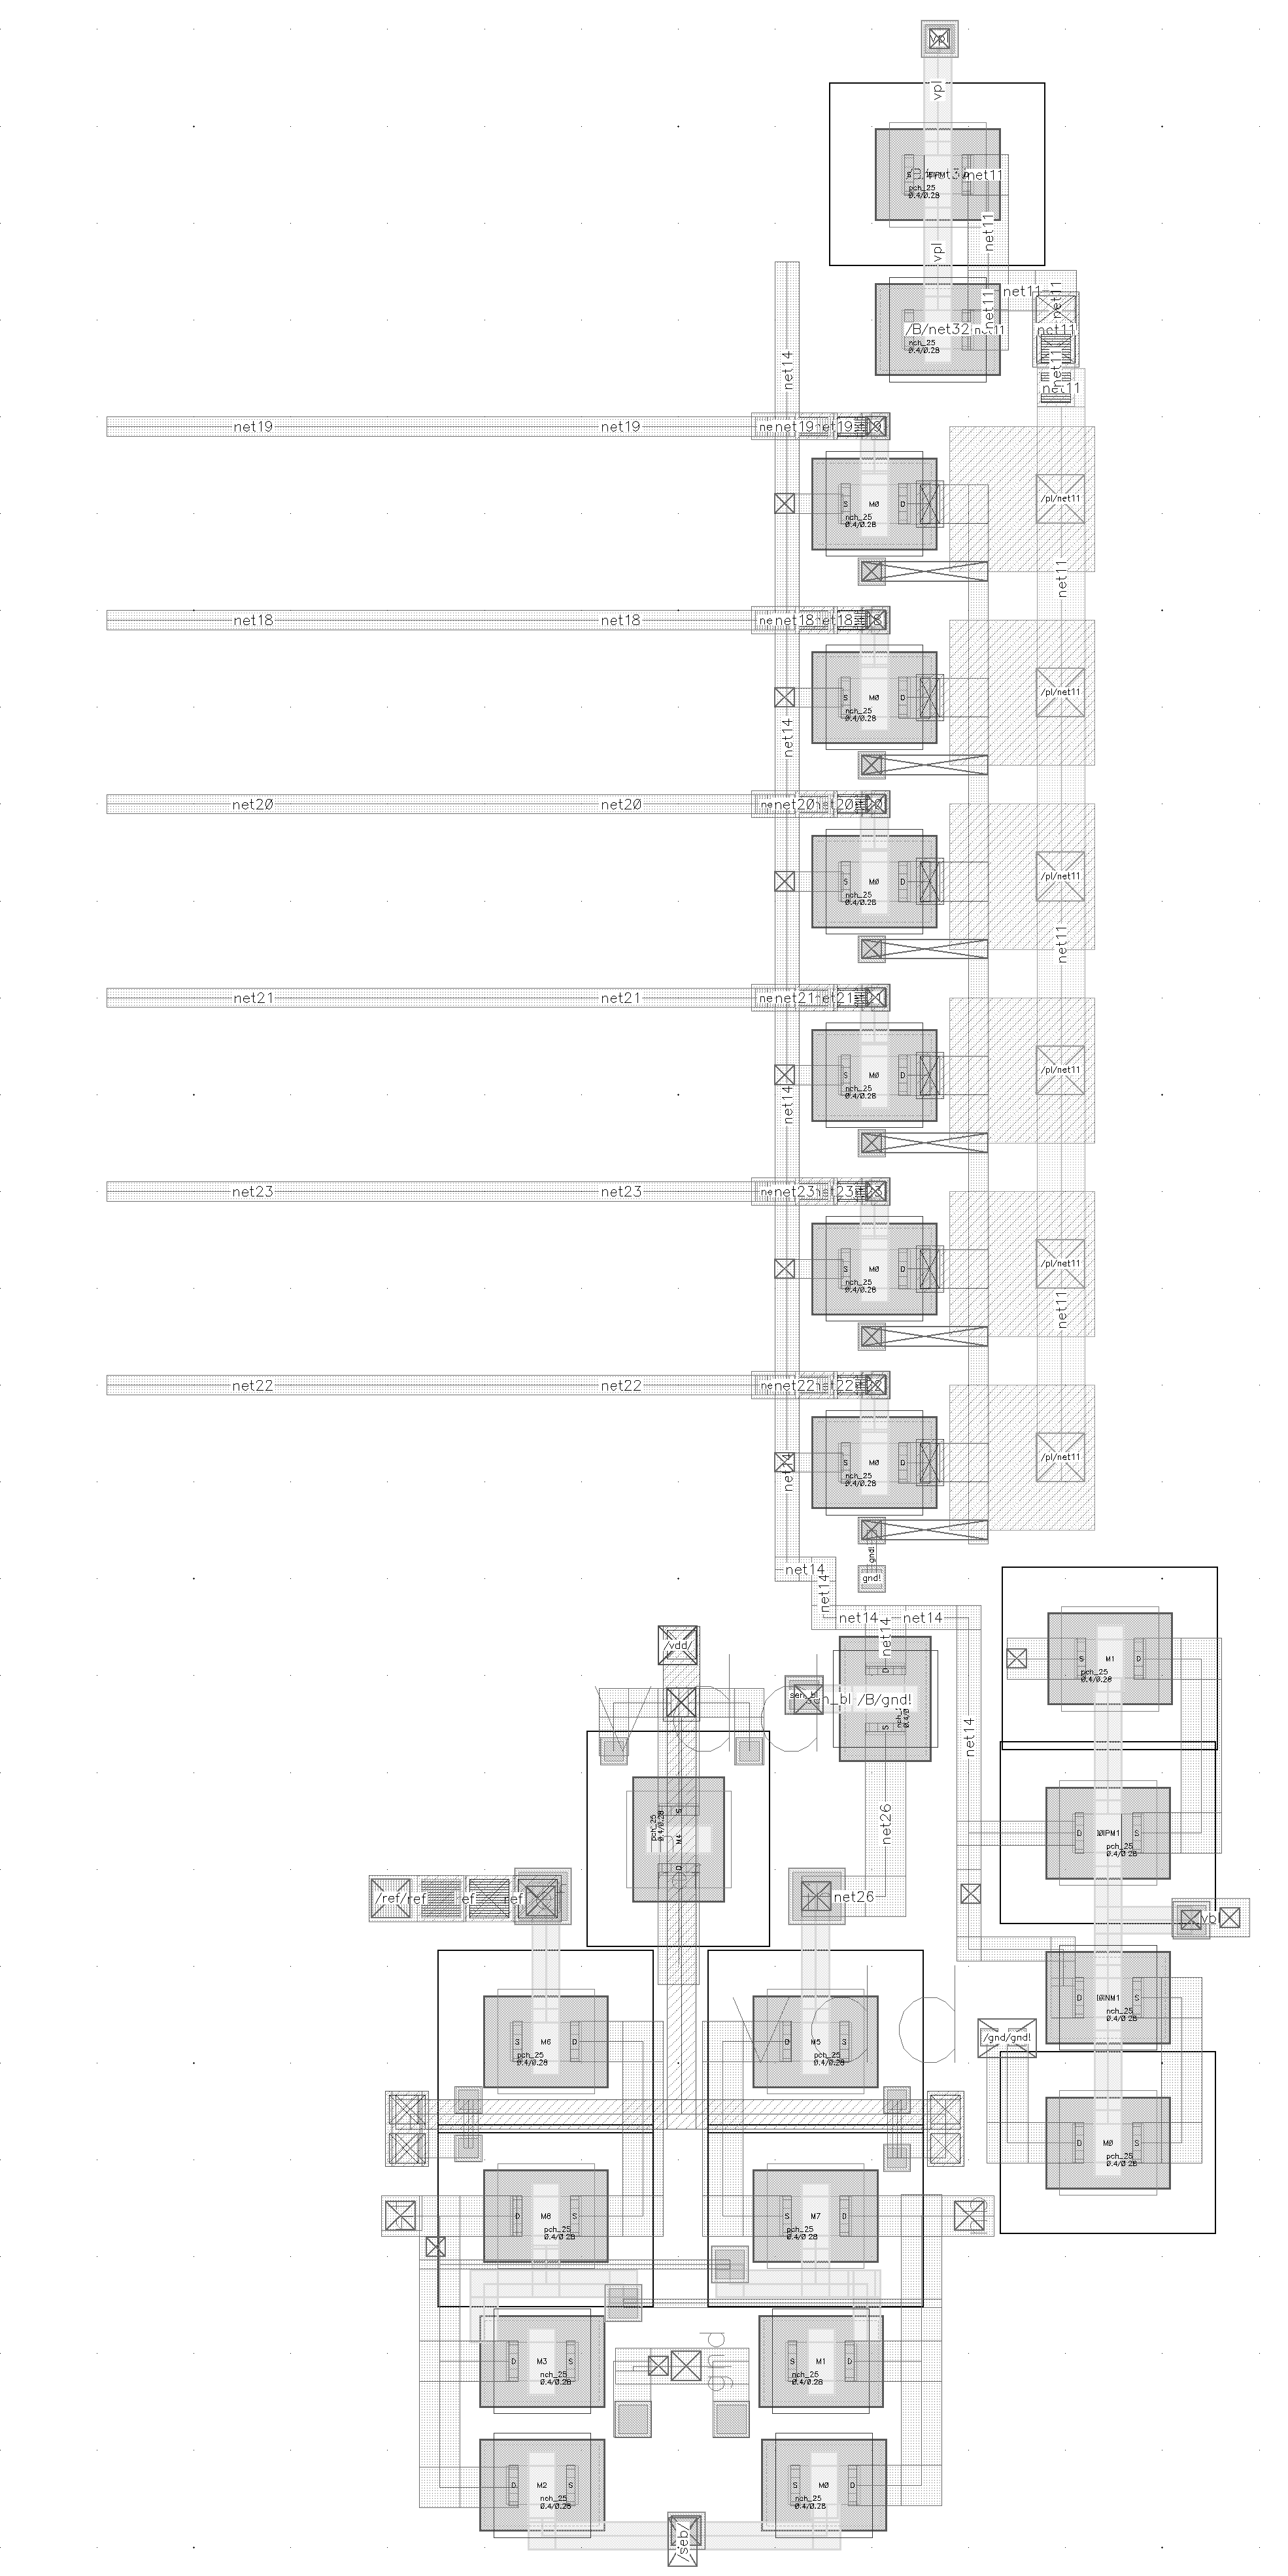
\includegraphics[width=0.8\linewidth]{array.png}
  \end{center}
  \caption{Топология столбца памяти}
  \label{pic:array_la}
\end{figure}
\newpage

\begin{thebibliography}{}
    \bibitem{Segneto_MIPT-I}  Improved Ferroelectric Switching Endurance of La-Doped $Hf_{0.5}Zr_{0.5}O_2$
Thin Films
Anna G. Chernikova, Maxim G. Kozodaev, Dmitry V. Negrov, Evgeny V. Korostylev,
Min Hyuk Park, Uwe Schroeder, Andrey M. Markeev,
	\bibitem{Segneto_MIPT-II}  Ultrathin $Hf_{0.5}Zr_{0.5}O_2$ Ferroelectric Films on Si
Anna Chernikova, Maksim Kozodaev, Andrei Markeev, Dmitrii Negrov, Maksim Spiridonov,
Sergei Zarubin, Ohheum Bak, Pratyush Buragohain, Haidong Lu, Elena Suvorova, Alexei Gruverman, and Andrei Zenkevich*

	\bibitem{Segneto_MIPT-III} La-doped $Hf_{0.5}Zr_{0.5}O_2$ thin films for high-efficiency electrostatic supercapacitors 
Maxim G. Kozodaev, Anna G. Chernikova, Roman R. Khakimov, Min Hyuk Park,
Andrey M. Markeev, and Cheol Seong Hwang4

	\bibitem{Segneto_MIPT-IV} Mitigating wakeup effect and improving
endurance of ferroelectric $HfO_2-ZrO_2$ thin
films by careful La-doping - Maxim G. Kozodaev , Anna G. Chernikova , Evgeny V. Korostylev , Min Hyuk Park , Roman R.
Khakimov , Cheol S. Hwang , and Andrey M. Markeev

	\bibitem {DRAM-I} Itoh, K.: VLSI Memory Chip Design. Springer 2001. ISBN 3-540-67820-4.
	\bibitem {DRAM-II} Itoh, K.: VLSI Memory Design. Tokyo (in Japanese): Baifukan 1994.
	
	\bibitem {IC-I} Razavi B. Design of Analog CMOS Integrated Circuits 
	\bibitem {IC-II} CMOS Circuit Design, Layout, and Simulation Third Edition R. Jacob Baker

	\bibitem {LATCH} NTUEE Electronics III: 17.1 Latches and Filp-Flops


   \bibitem {CFRAM} Takashima, D. et al.: High-Density Chain Ferroelectric Random-Access Memory (CFRAM). Symp.VLSI Circuits Dig.Tech.Papers (1997), pp. 83-84.
   
   \bibitem {FRAM} Advanced Circuit Design of
Gigabit-Density Ferroelectric
Random-Access Memories Jürgen Thomas Rickes aus Neuwied  

   \bibitem {carlo} Demir, Alper \& W. Y. Liu, Edward \& Sangiovanni-Vincentelli, Alberto. (1996). Time-Domain Non-Monte Carlo Noise Simulation for Nonlinear Dynamic Circuits with Arbitrary Excitations. Computer-Aided Design of Integrated Circuits and Systems, IEEE Transactions on. 15. 493 - 505. 10.1109/43.506137

	\bibitem {ssd} 9200 NVMe(TM) SSDs
MTFDHAL1T6TCU, MTFDHAL1T9TCT, MTFDHAL3T2TCU,
MTFDHAL3T8TCT, MTFDHAL6T4TCU, MTFDHAL7T6TCT,
MTFDHAL8TATCW, MTFDHAL11TATCW datasheet
    \bibitem {patent}  патент АС СССР 690564
	\bibitem {ferro} Physics of ferroelectrics PBLittlewood January 27, 2002
	\bibitem {lib:c_bl} Yamada, J. et al.: A 128kb FeRAM Macro for a Contact/Contactless Smart Card Microcon-troller. ISSCC Dig.Tech.Papers (2000), pp. 270-271.

	\bibitem {fram18} Chung, Y., Jeon, B.-G., and Suh, K.-D.: A 3.3-V, 4-Mb Nonvolatile Ferroelectric RAM with Selectively Driven Double-Pulsed Plate Read/Write-Back Scheme. IEEE J.of Solid-State Circuits vol. 35 (2000) no. 5, pp. 697-704.

\end{thebibliography}



\end{document}